% ===================================================================================================
%                                                 |                                                 |
%                                                 |                                                 |
% -------------------------------------------- SECTION ---------------------------------------------|
%                                                 |                                                 |
%                                                 |                                                 |
% ===================================================================================================
\section{Collective learning in robotics\TODO}
%---
\begin{figure*}[ht!]
	\centering
	\hspace*{\fill}
	\subfloat[]{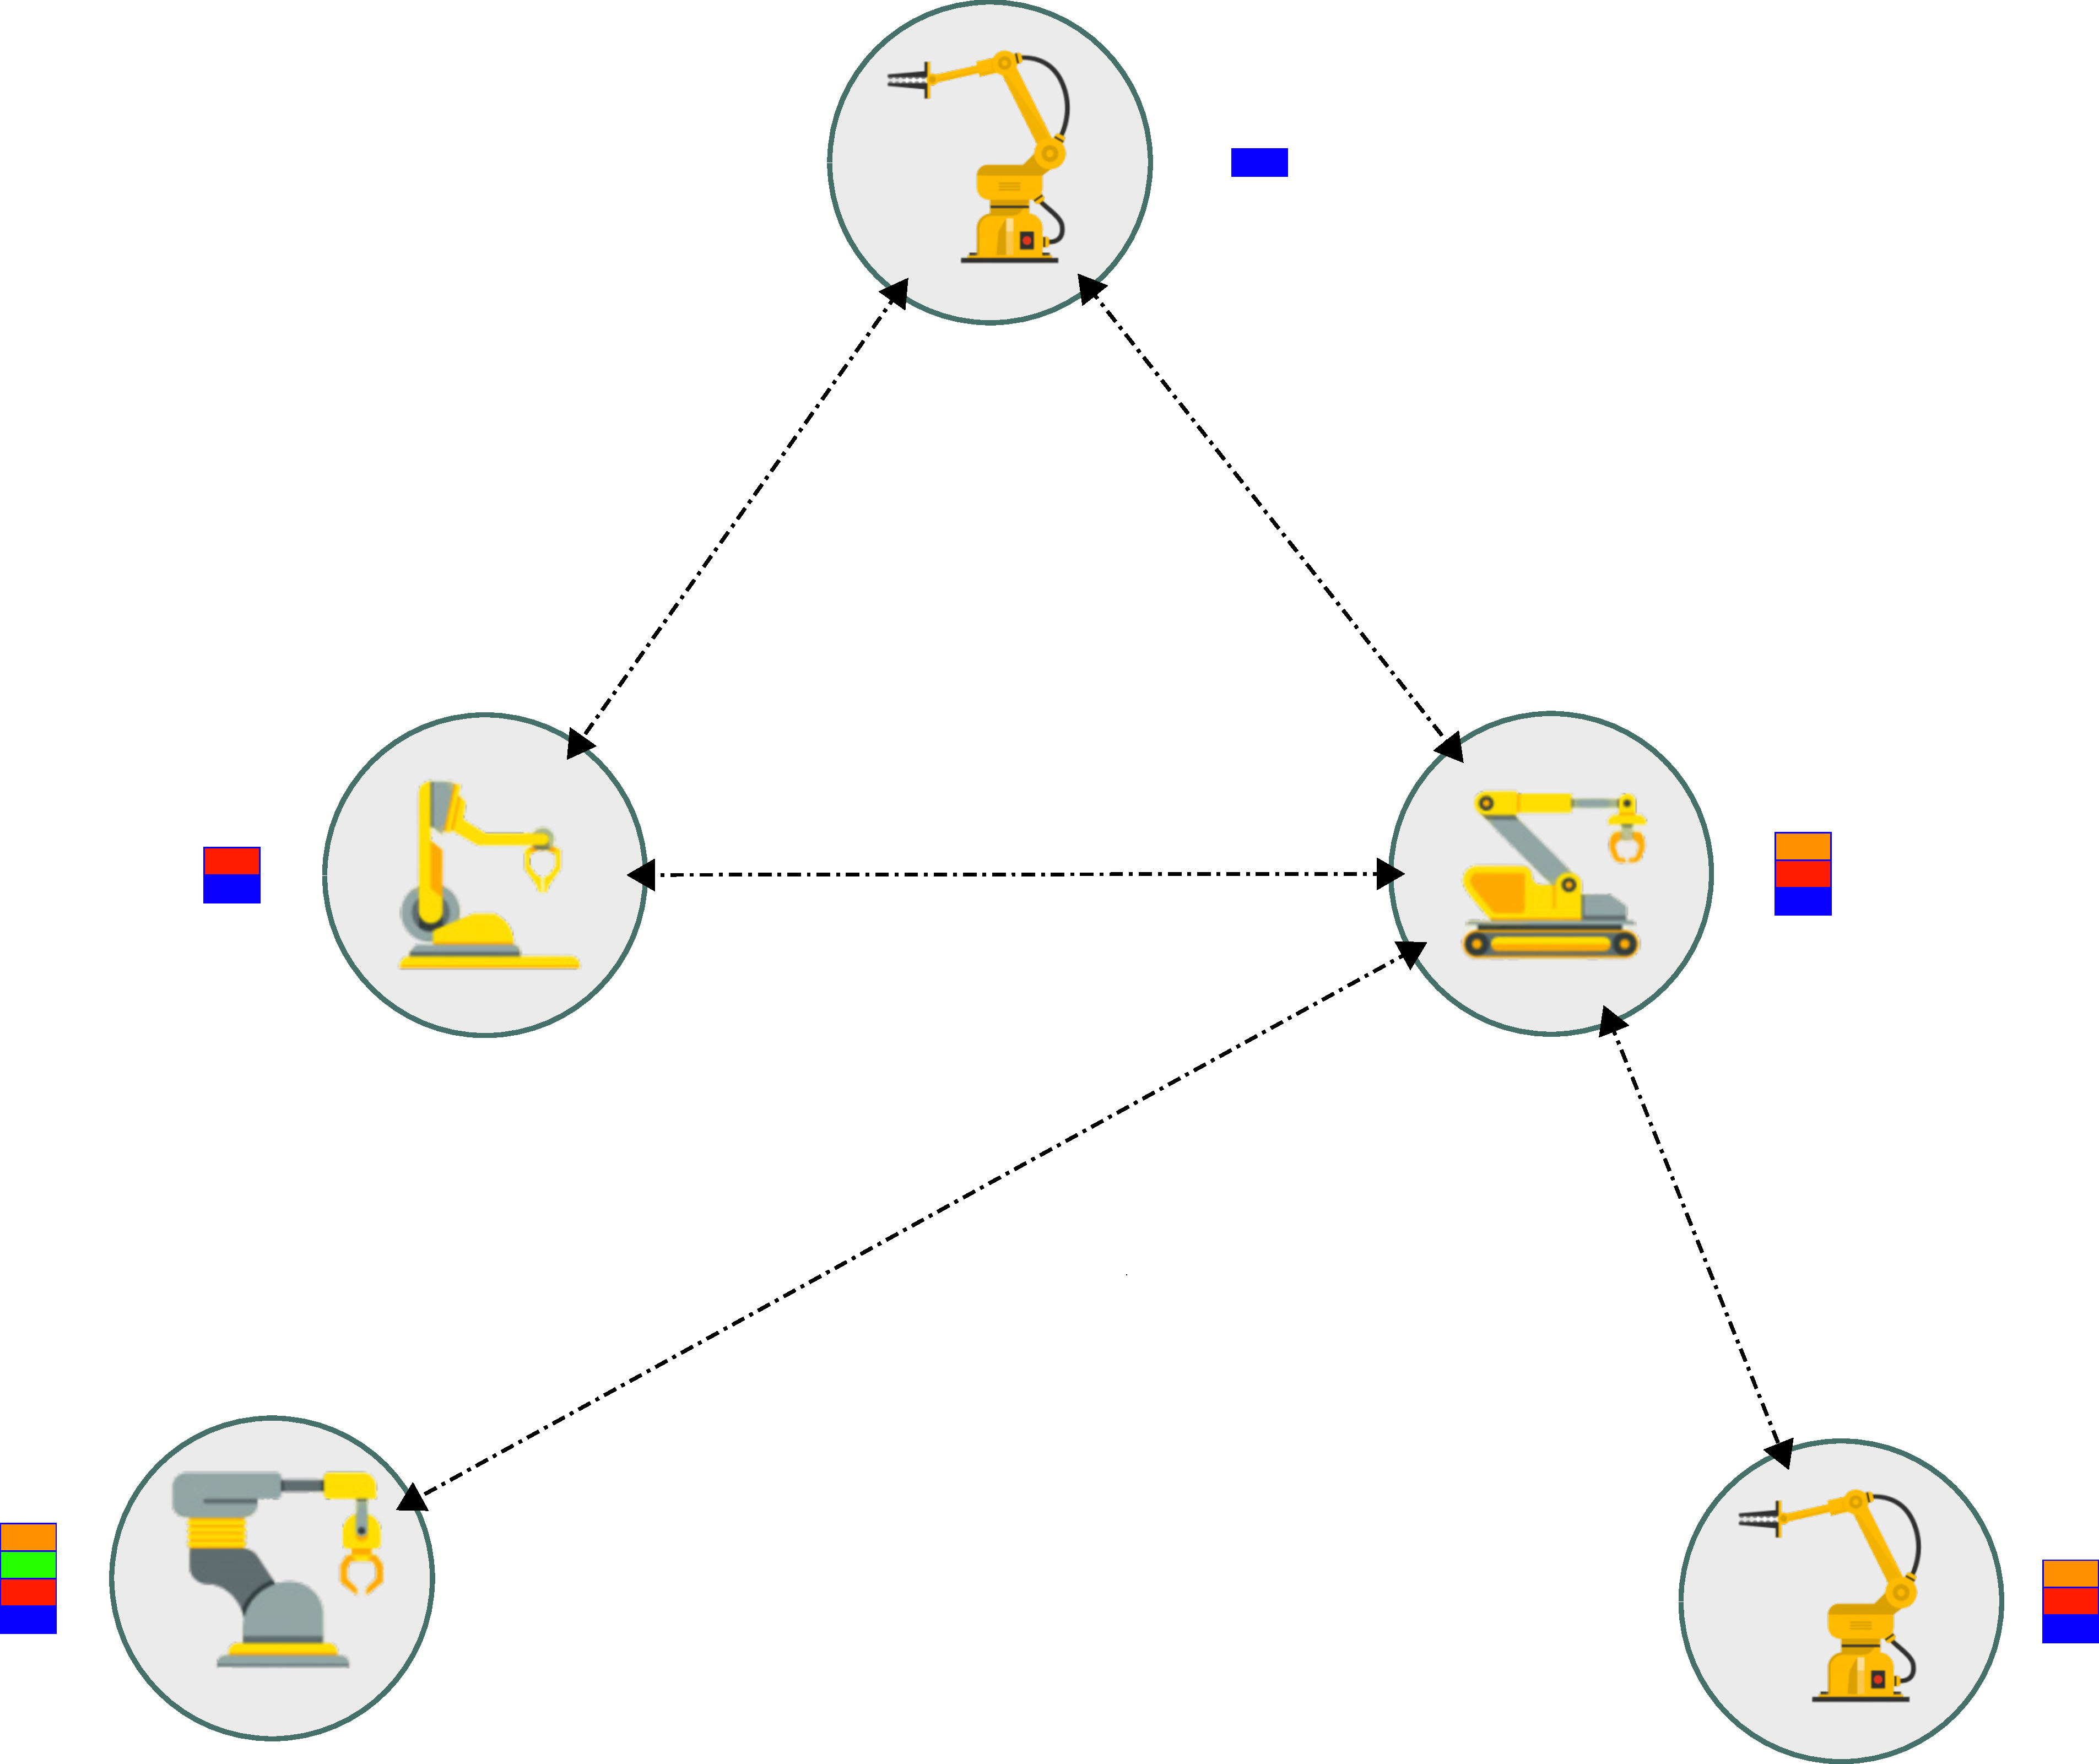
\includegraphics[width= 0.90\columnwidth]{fig/collective_learning_v4.pdf} \label{fig:isolated_learning}}
	%\hspace*{\fill}
	\hfill
	\subfloat[]{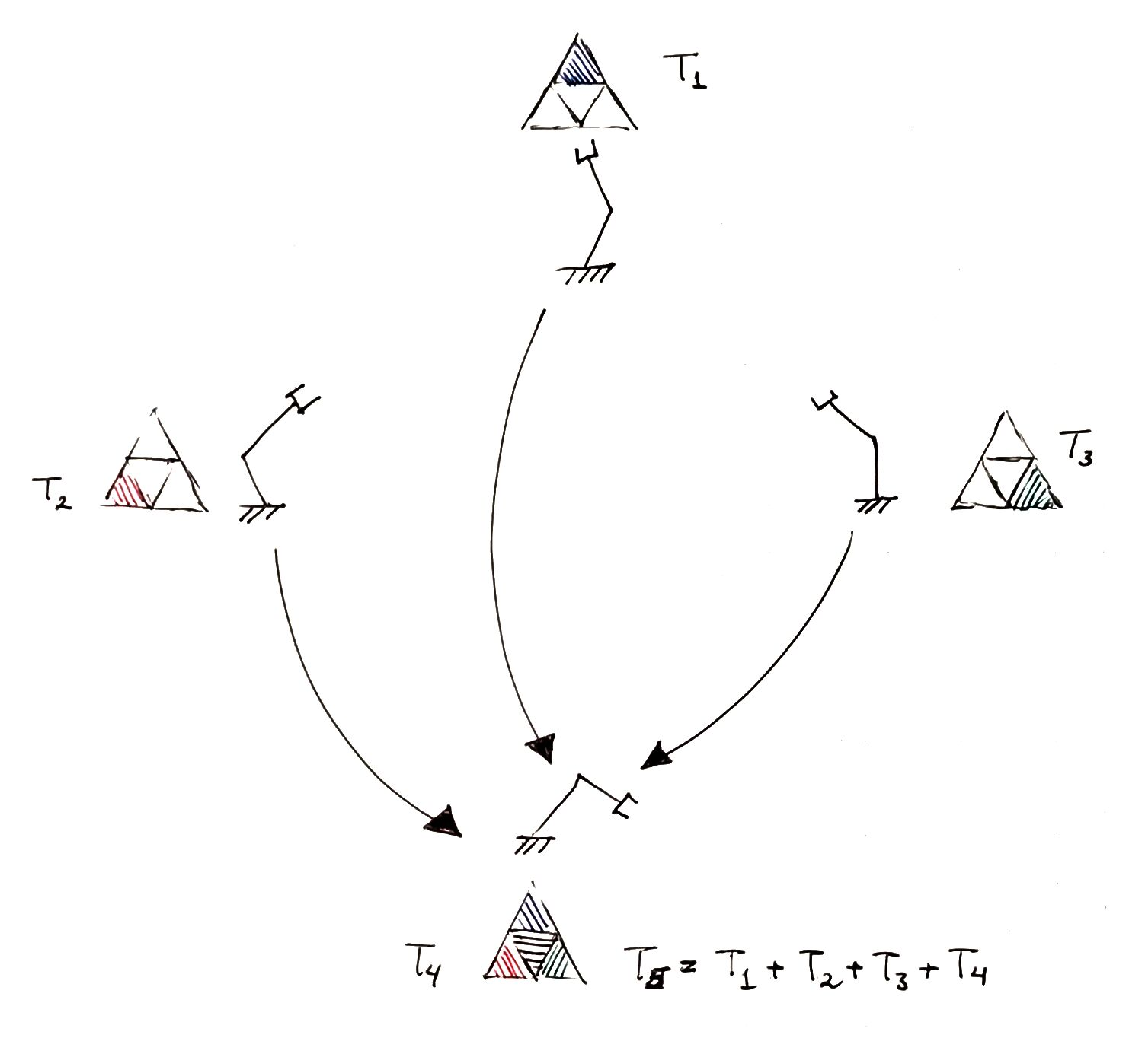
\includegraphics[width= 0.80\columnwidth]{fig/collective_learning_concept.pdf} \label{fig:collective_learning}}
	\hspace*{\fill}
	\caption[] {\label{fig:learning_paradigms} Knowledge building. }
\end{figure*}
%---
\begin{figure*}[ht!]
	\centering
	\hspace*{\fill}
	\subfloat[]{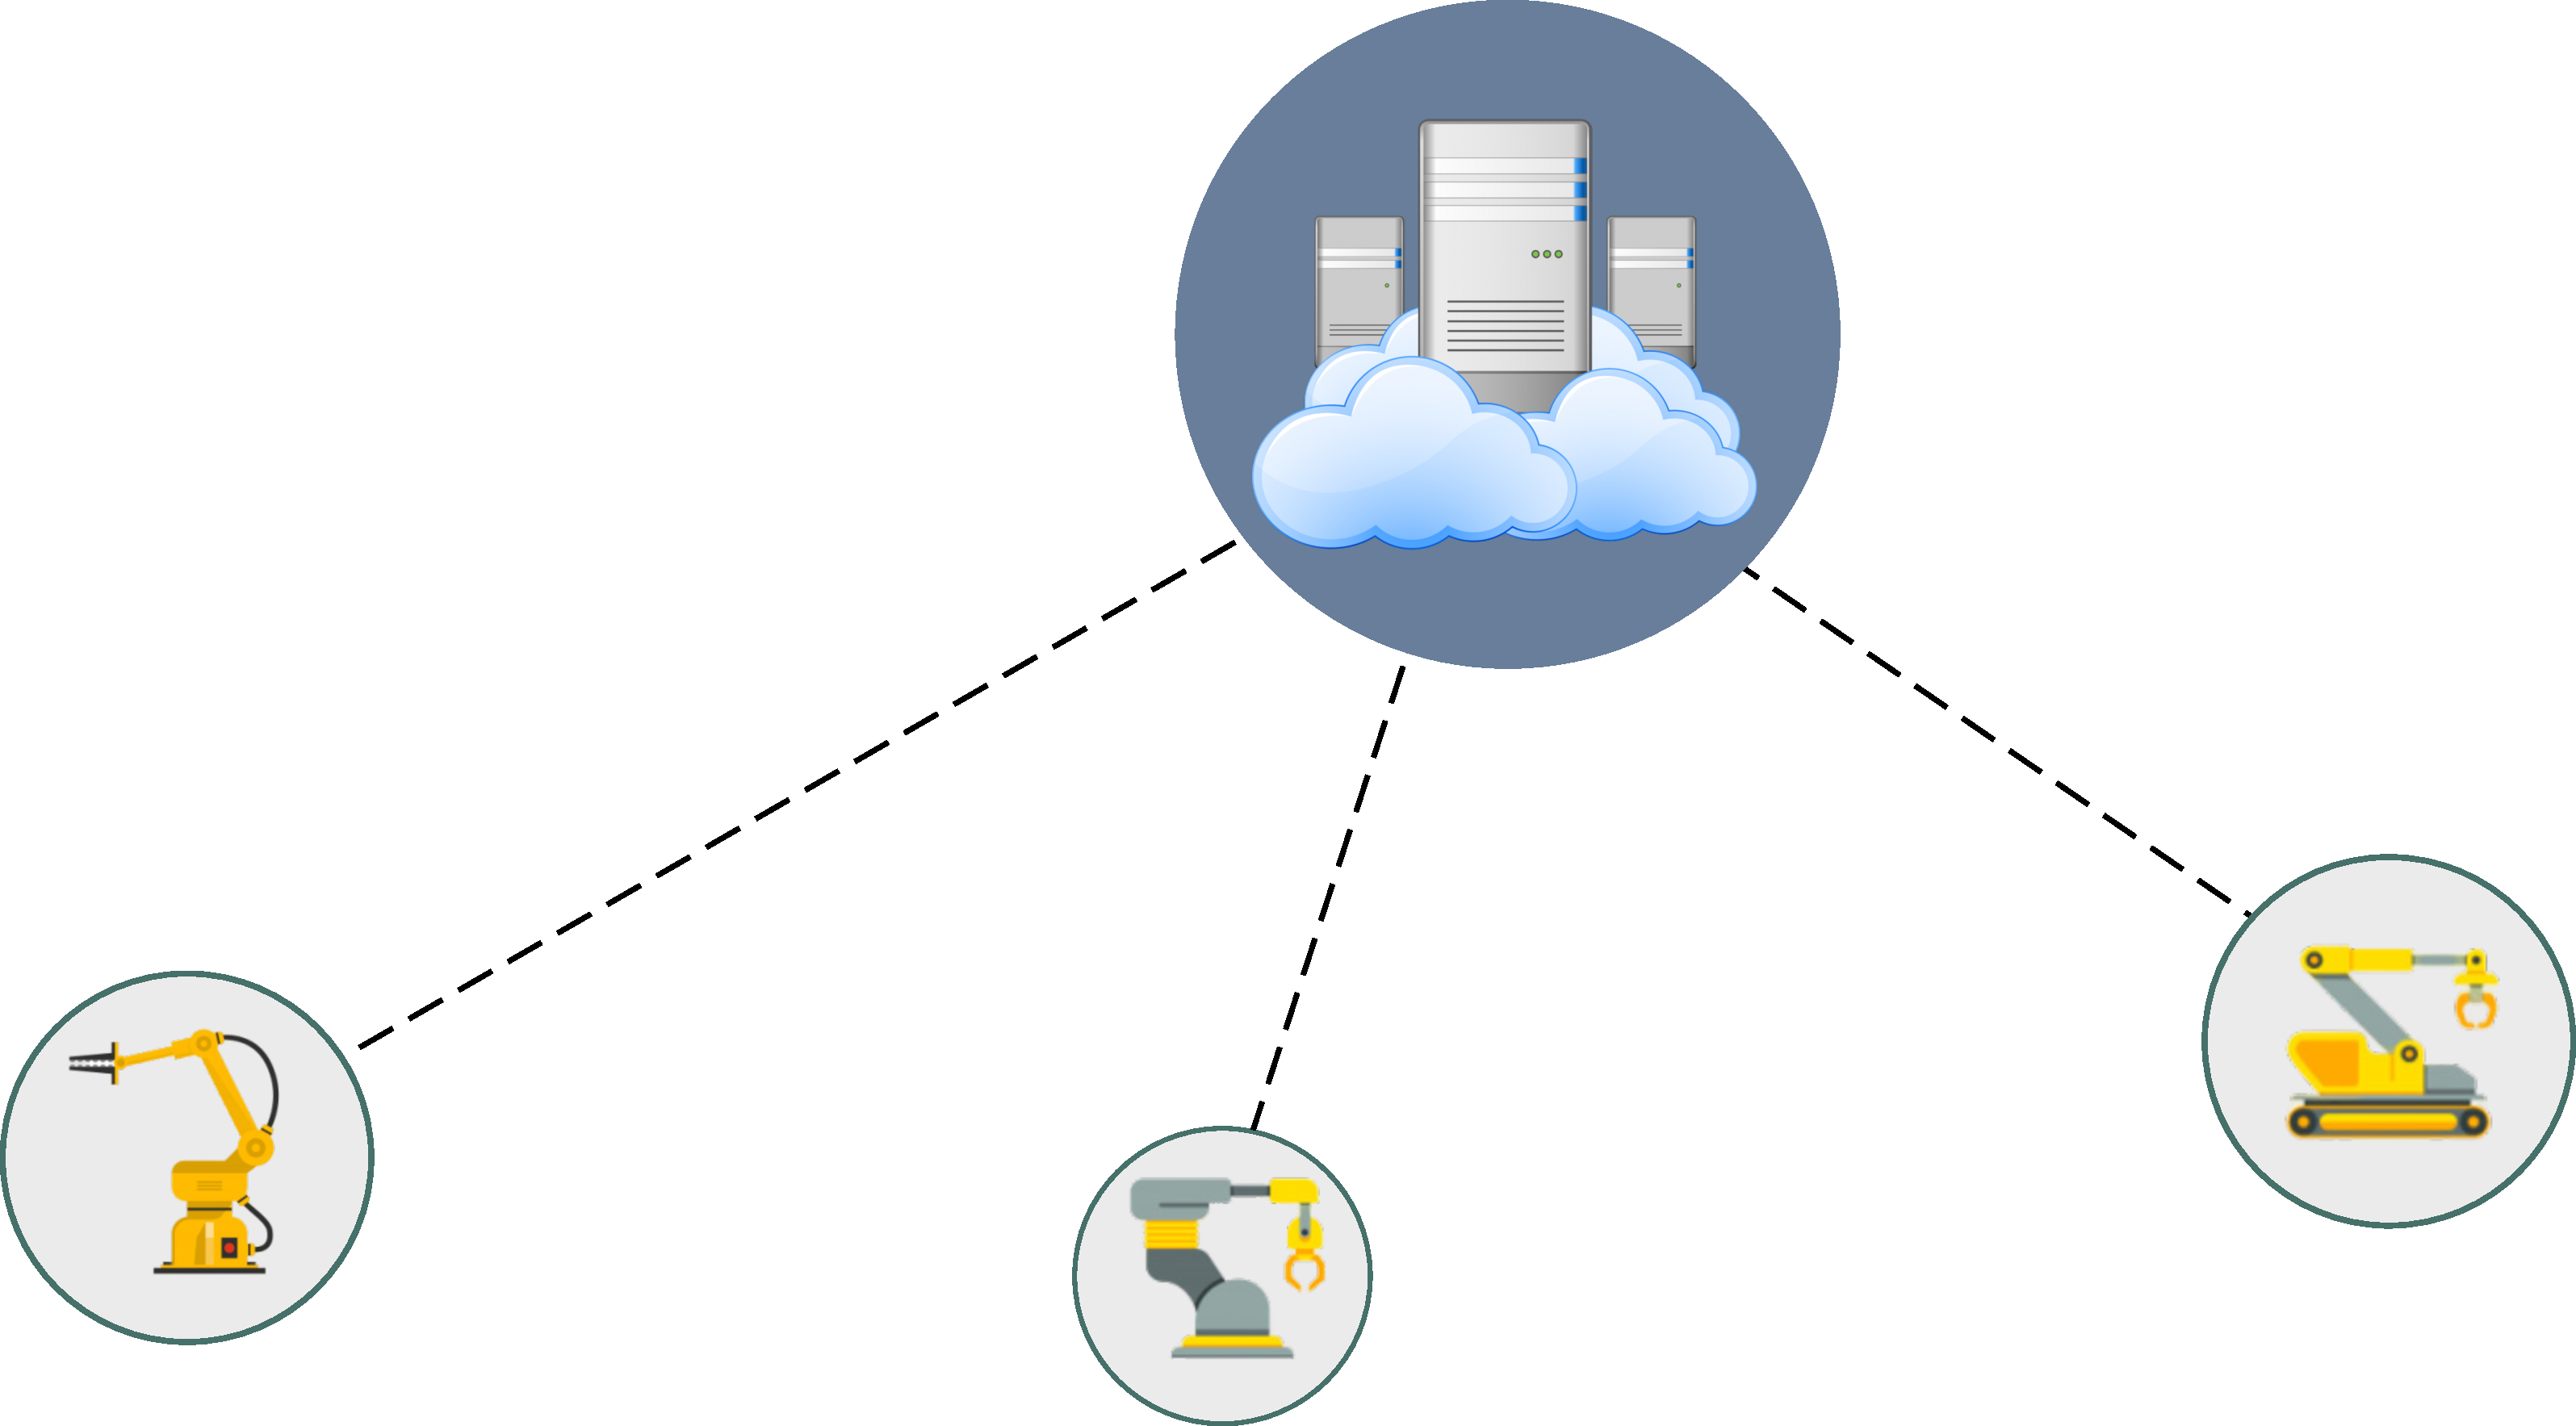
\includegraphics[width= 0.90\columnwidth]{fig/isolated_learning.pdf} \label{fig:isolated_learning}}
	%\hspace*{\fill}
	\hfill
	\subfloat[]{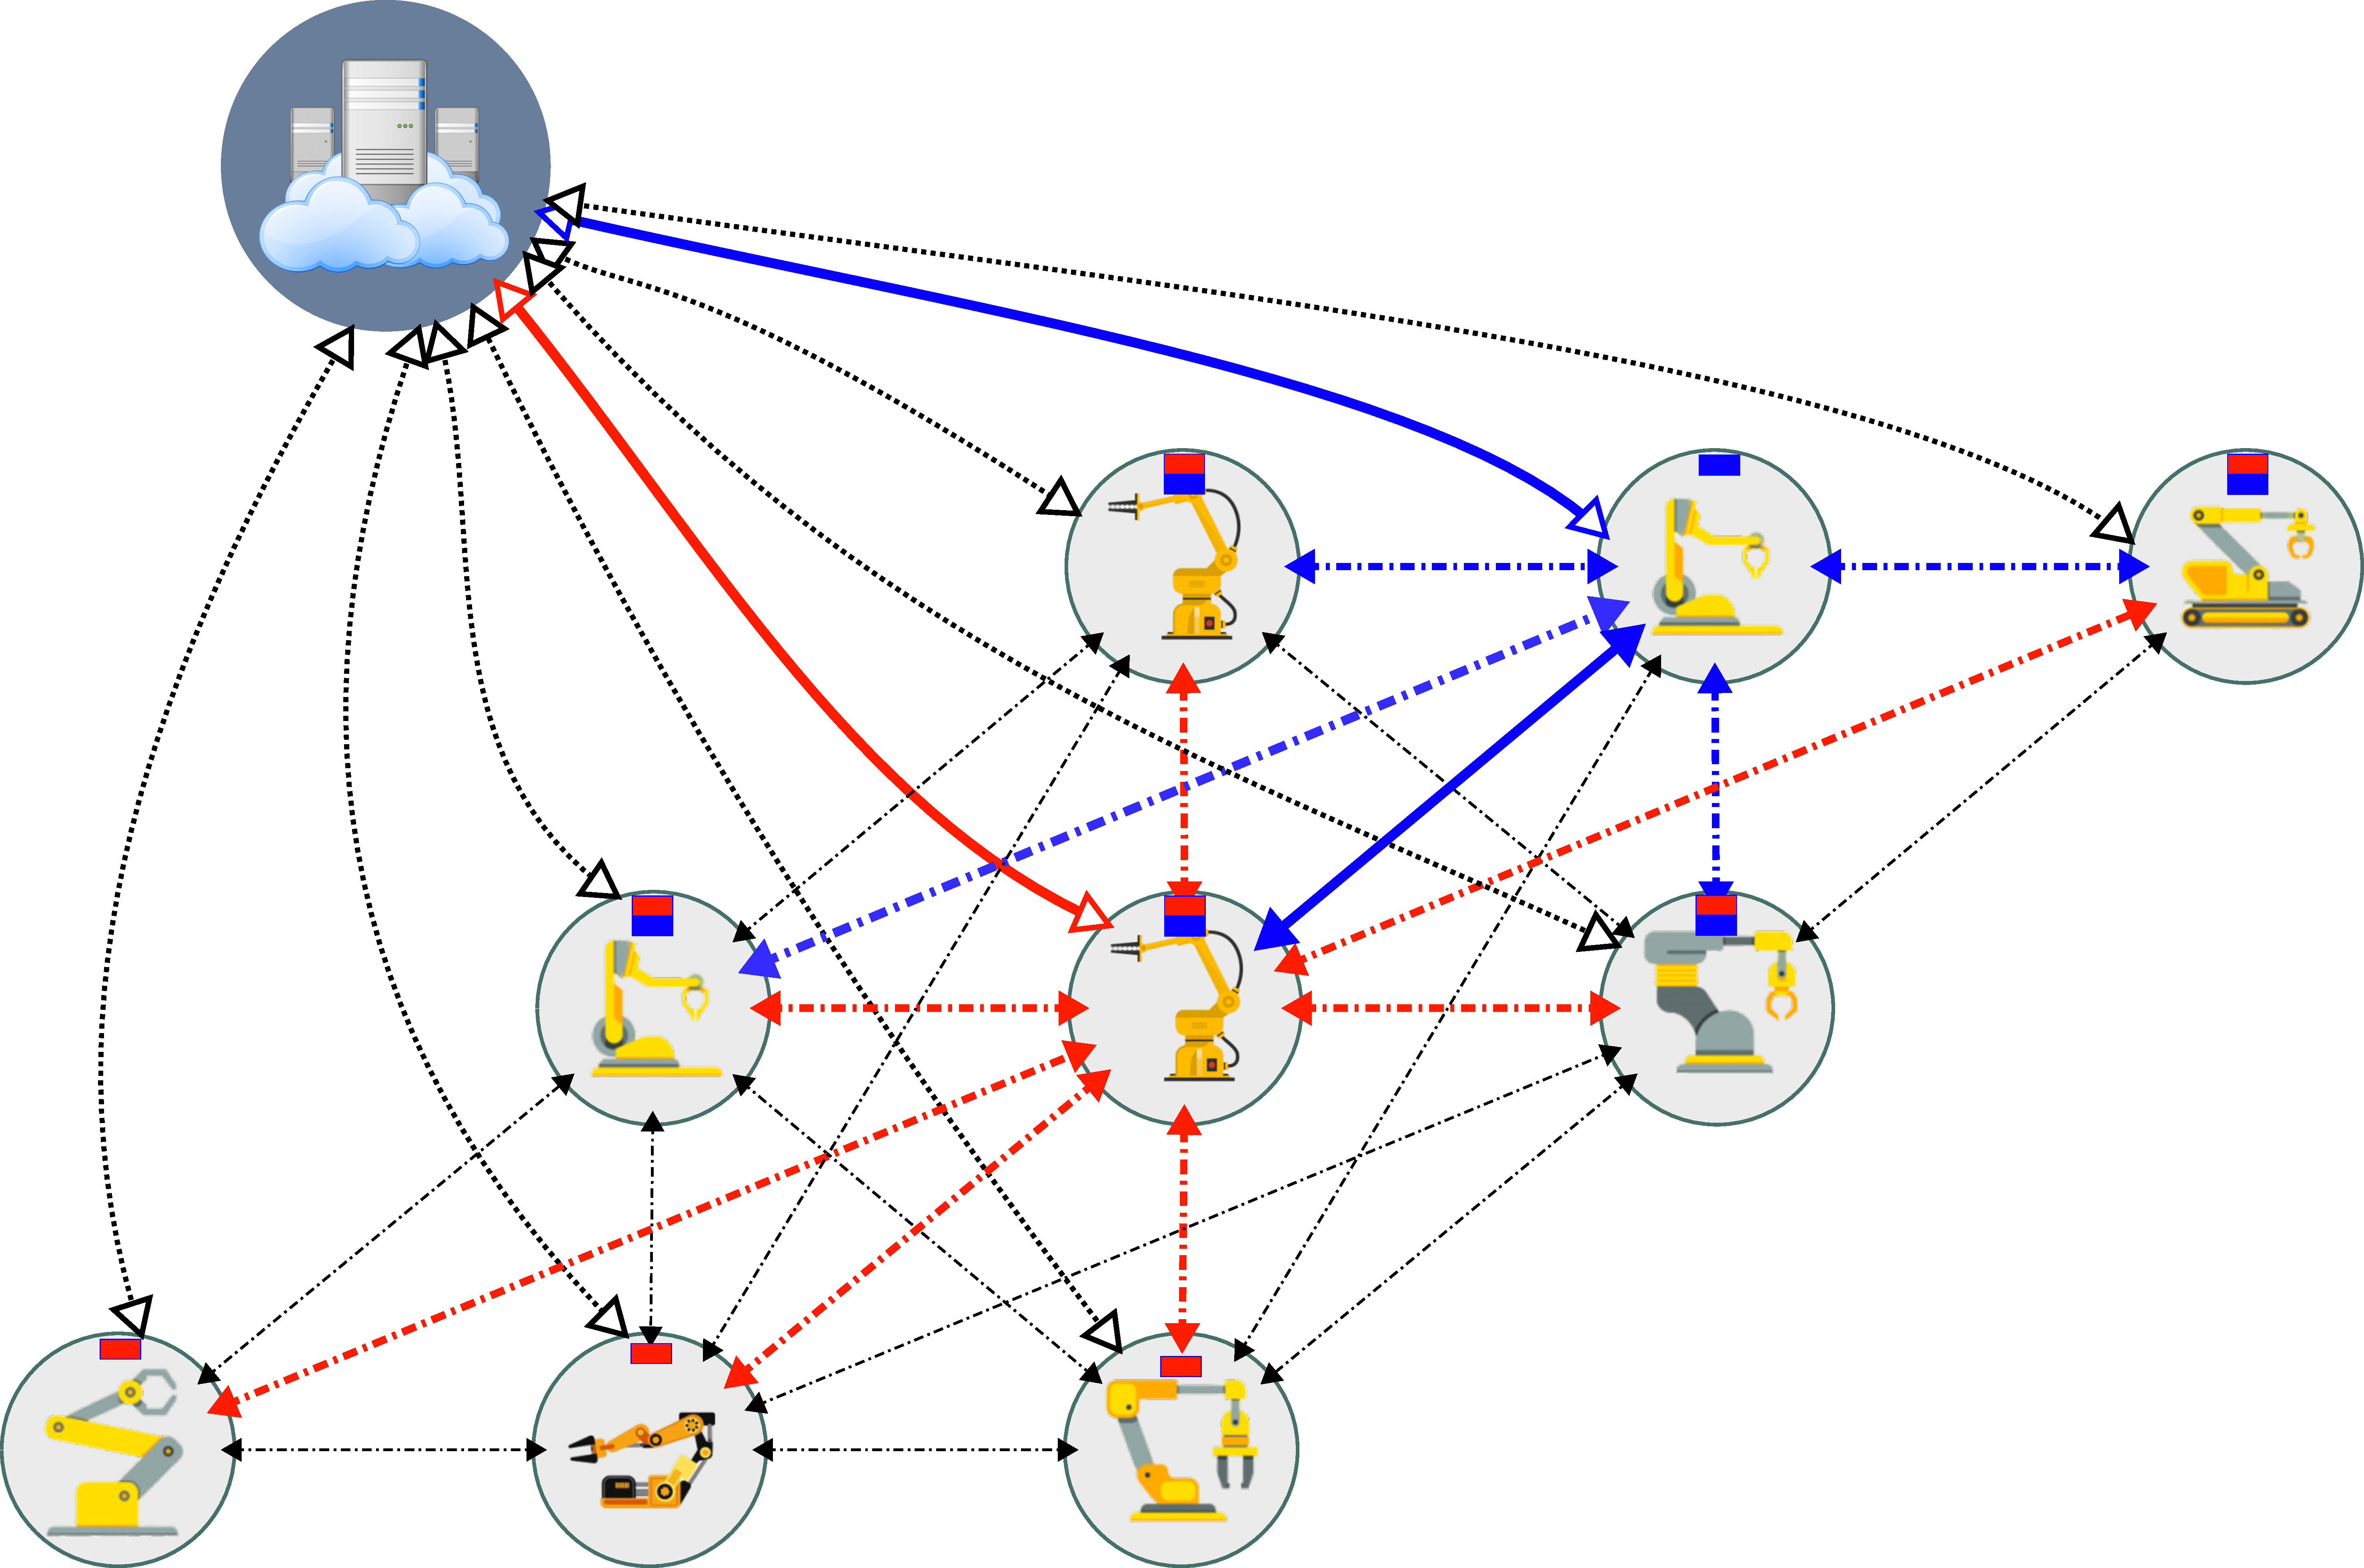
\includegraphics[width= 0.90\columnwidth]{fig/collective_learning_v3.pdf} \label{fig:collective_learning}}
	\hspace*{\fill}
	\caption[] {\label{fig:learning_paradigms} Learning paradignms: \subref{fig:isolated_learning} transfer learning and \subref{fig:collective_learning} collective learning. }
\end{figure*}
%---
In Transfer Learning, one of the most basic premises is that a given learning system can leverage knowledge to solve a task from previous experiences with similar tasks. It is common to see in the literature that the learner is composed of a single-agent and, therefore, it is only possible to learn from the own agent's previous data. A logical way to improve the learning speed is to use a multi-agent setting. To outperform the single-agent case it is expected that some form of parallelization is explored, the most simple approach is to have a centralized learning model and distribute different attempts among all agents, this would, potentially, already accelerate the learning by the number of agents in the system. If, for example, some smart exploration and task segmentation scheme is used, the acceleration can increase by many times more. 

Collective Learning is the umbrella term used to describe the subset of learning algorithms that can leverage on multi-agent sets with a centralized learning model. The general high-level goal is that agents who are learning similar tasks in parallel can share common knowledge despite not yet been able to accomplish their tasks. The idea is that each agent experience can aggregate in the learning process of another. 

Let $ \left\lbrace r_i \right\rbrace_{i=1}^{N_r} $ be a set of robotic agents that defines a community of robots. In collective learning, the different robotic agents $ r_i $ develop and accumulate dynamical a common mind (body of knowledge) via networked interactions where individual experience, knowledge and skills are disseminated to all the other elements in the collective. Information flows vertically as previous knowledge is passed on, as well as the horizontally by sharing concurrent experience between agents, Via these mechanisms, knowledge can be replicated, complimented and further developed. We take from \cite{Garavan2012CollectiveLearning} two notions central in collective learning that are applicable to the robots:
\begin{enumerate}
	\item Capability to restructure and meet changing conditions
	\item Aggregation of skills, knowledge, and behaviors
\end{enumerate}

Collective learning contrasts with the previously discussed transfer learning in that a single agent $ r_i $ can aggregate only so much knowledge via trial and error and is limited by a sequential learning structure. Learning collectively, on the other hand, enforces parallelization of knowledge acquisition via the concurrent learning and sharing of all agents as they acquire new skills, knowledge. Moreover, collective learning involve not only the information acquisition, but also how this information is brought to use to form and develop knowledge. 

%---
%\begin{figure}[!ht]
%	\centering
%	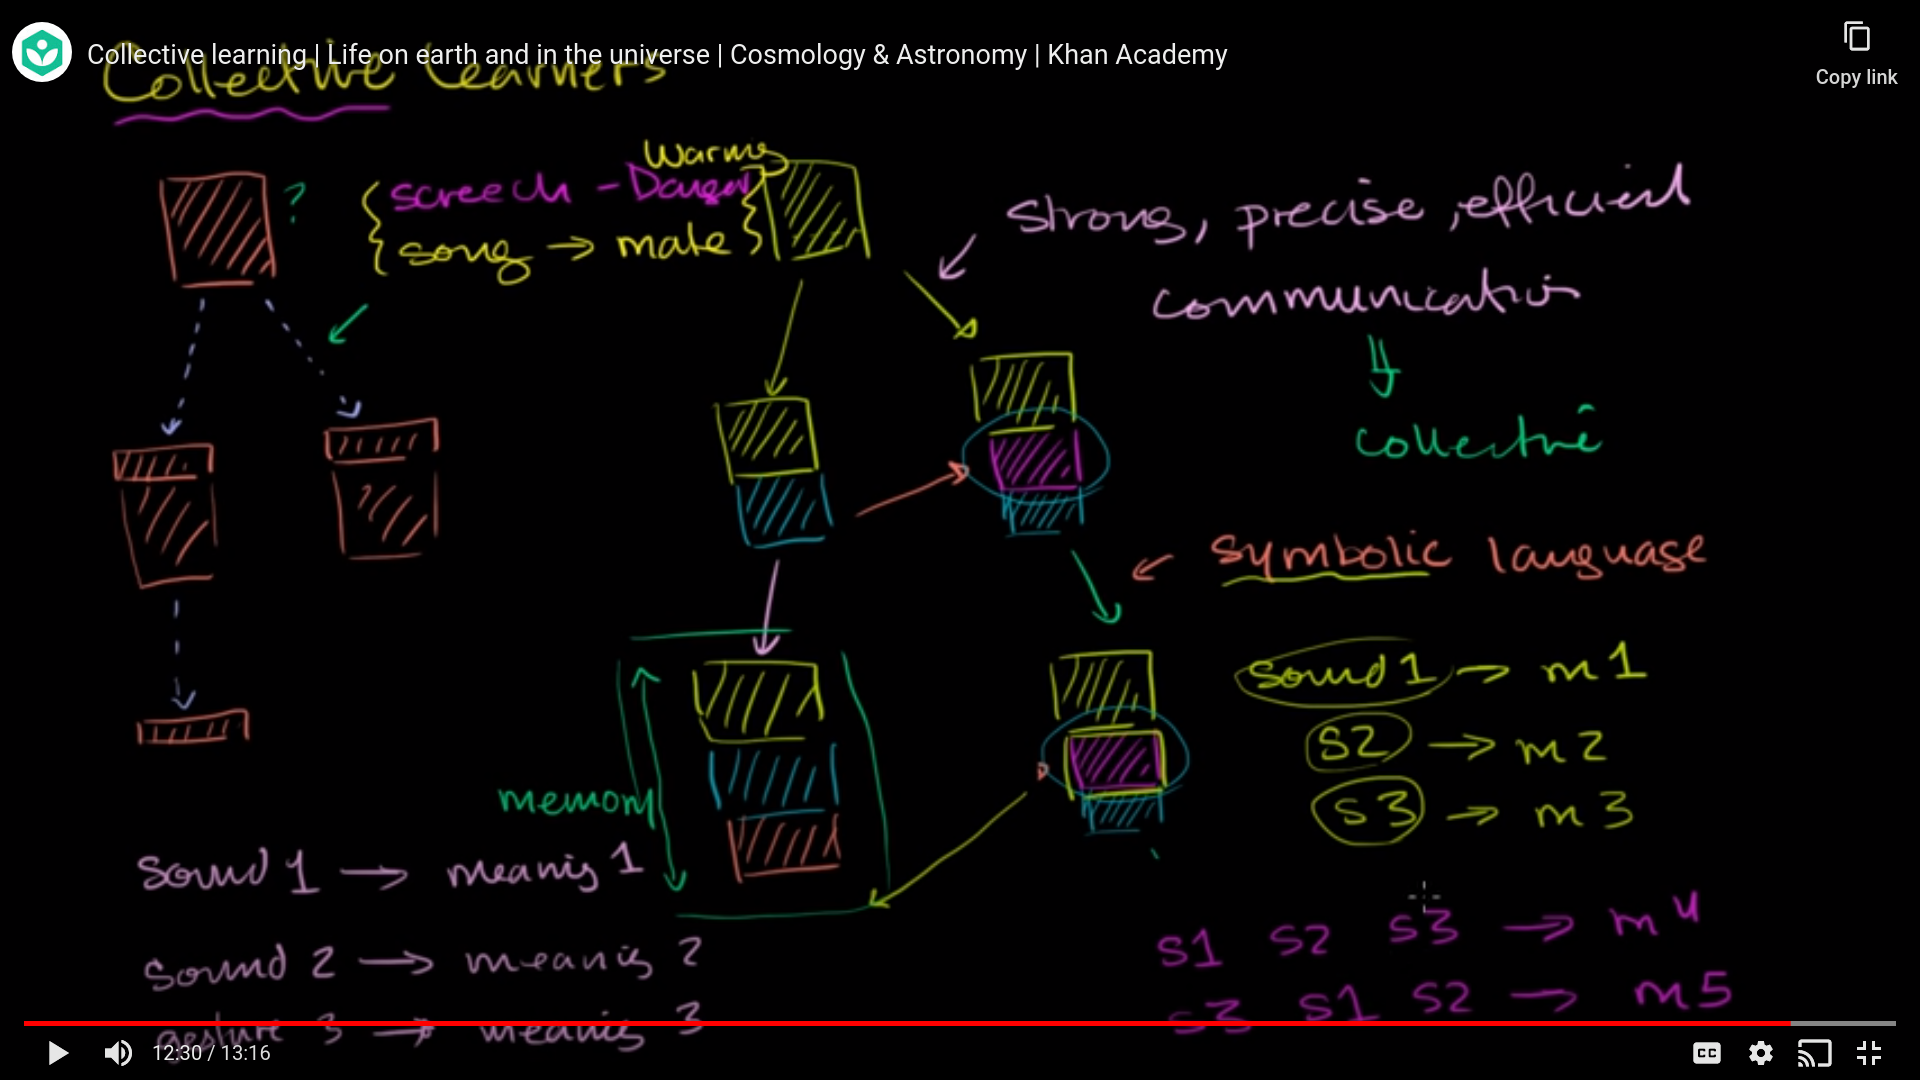
\includegraphics[width=1\columnwidth]{fig/collective_learning.png}
%	\caption{How knowledged is transferred, shared, and developed in a collective}
%	\label{fig:collective_learning}
%\end{figure}

%\begin{figure}[!ht]
%	\centering
%	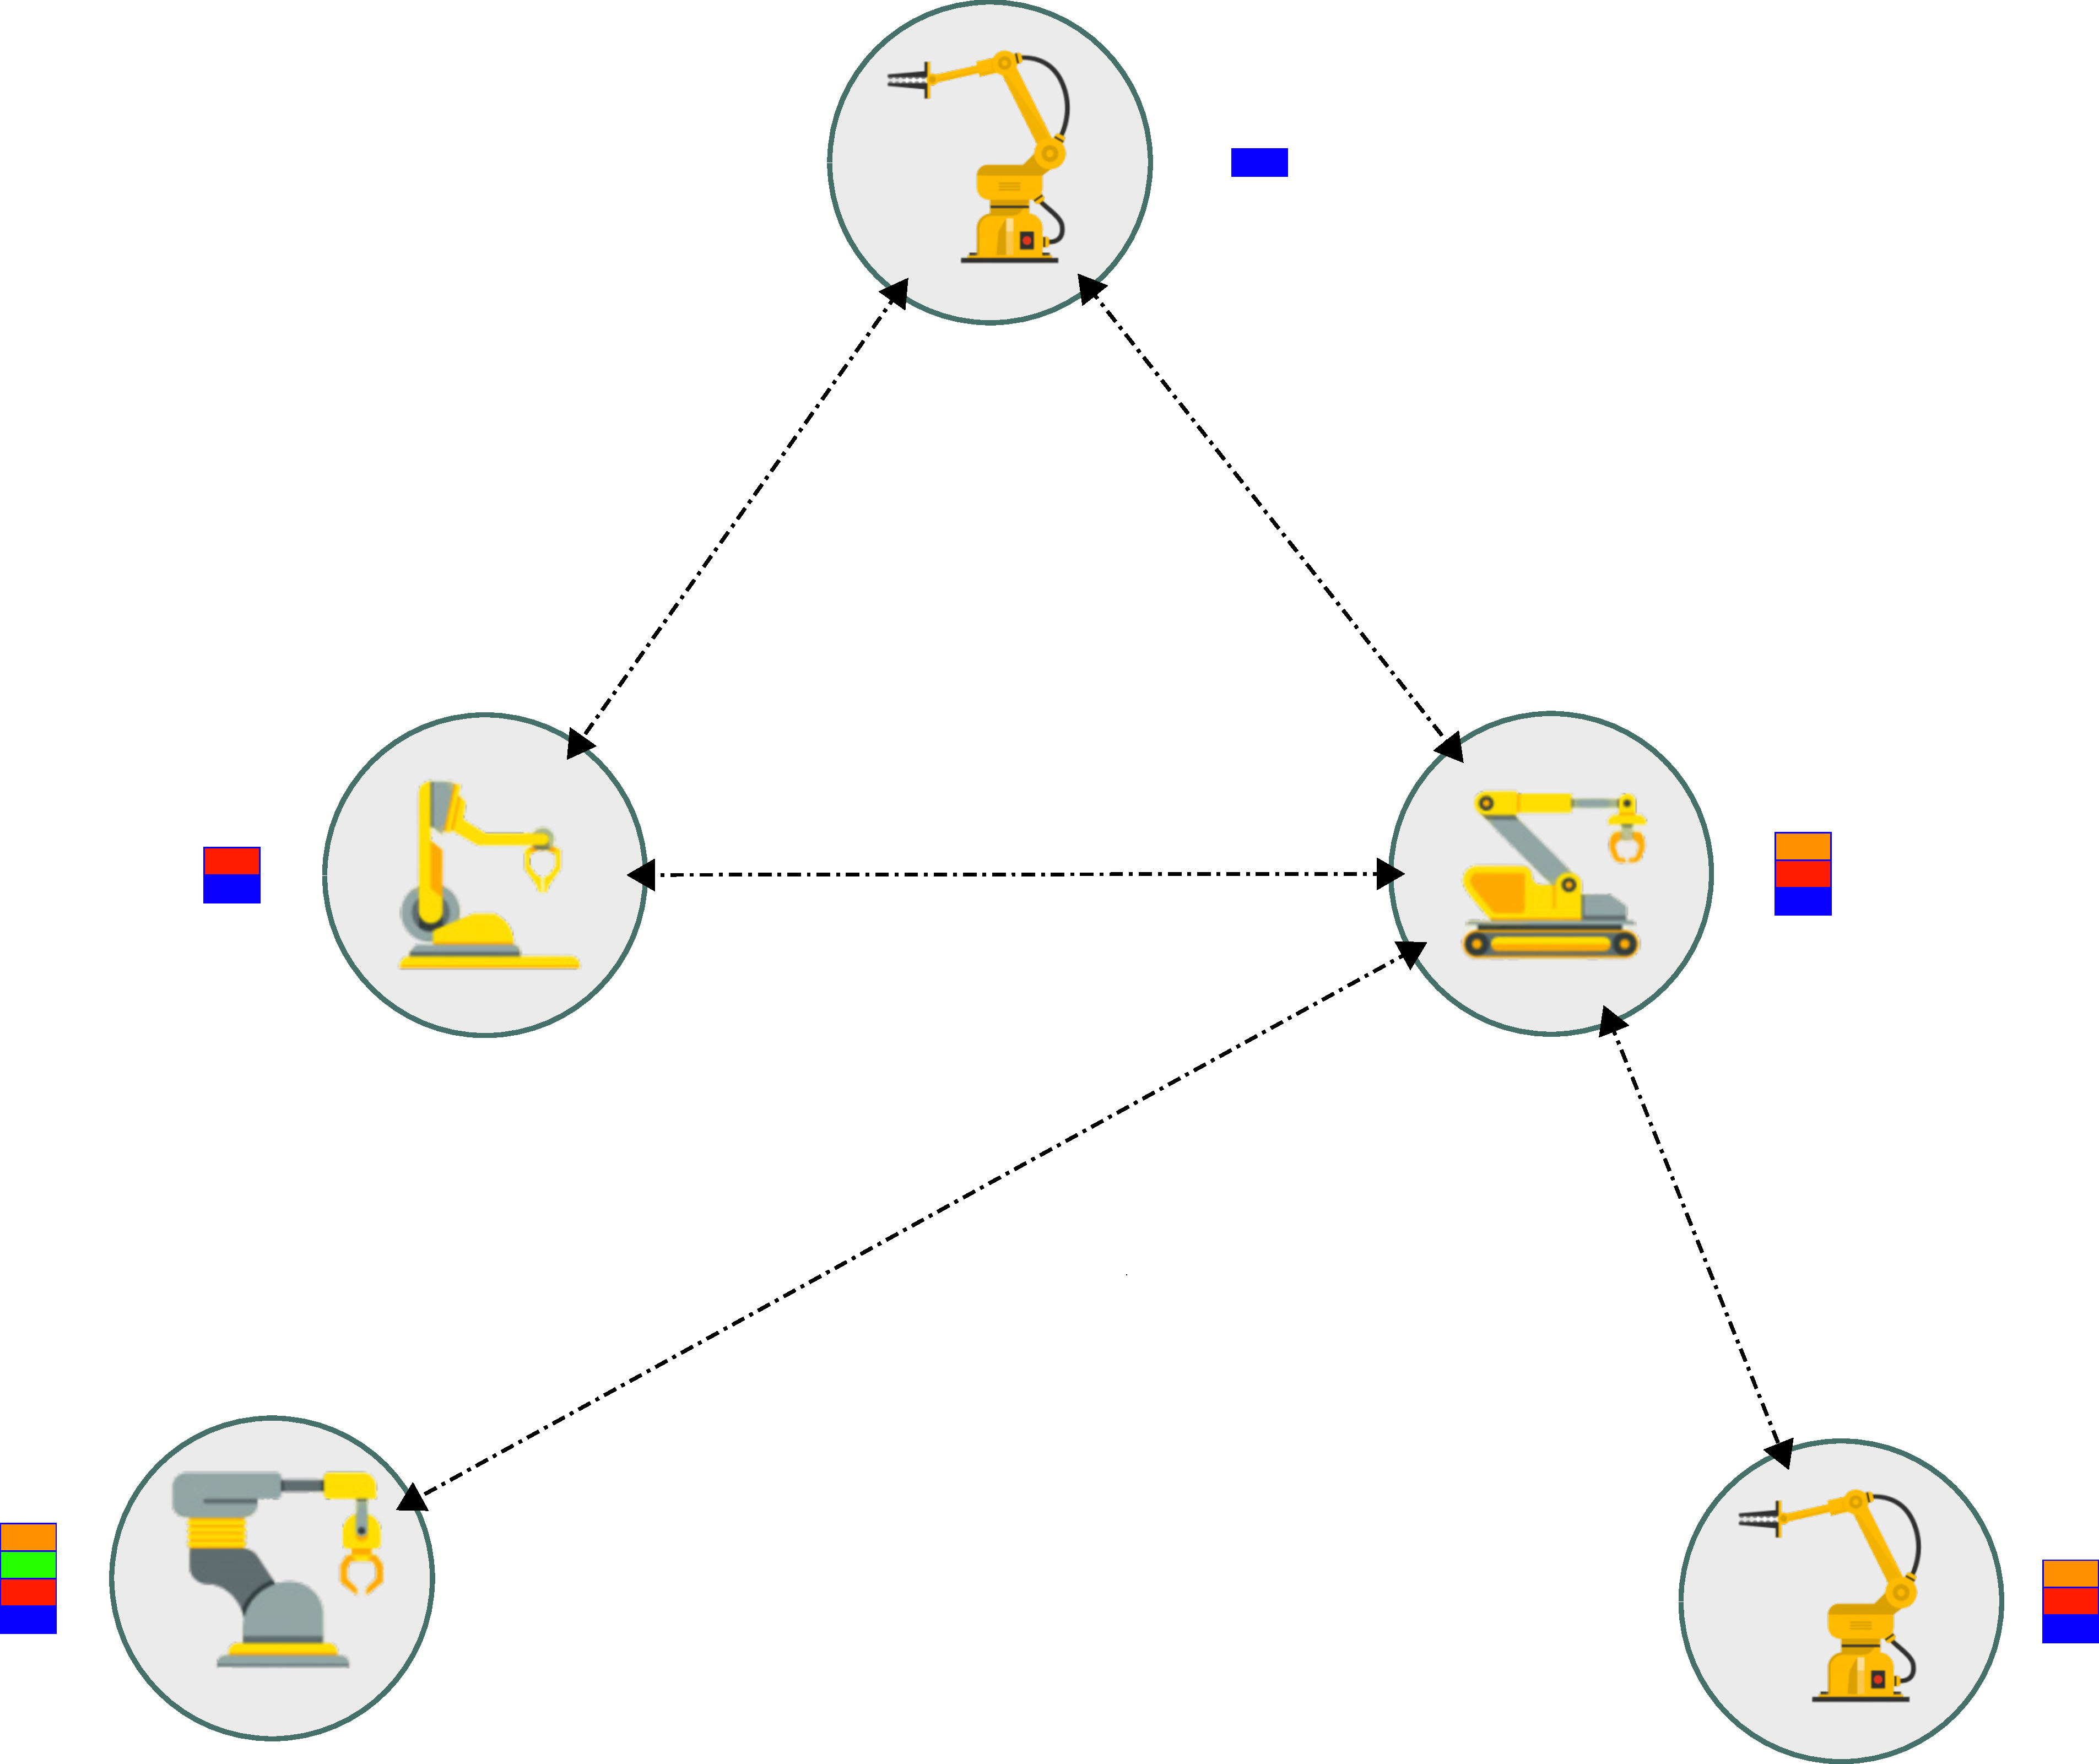
\includegraphics[width=1\columnwidth]{fig/collective_learning_v4.pdf}
%	\caption{How knowledged is transferred, shared, and developed in a collective}
%	\label{fig:collective_learning_v4}
%\end{figure}




%\begin{figure}[!ht]
%	\centering
%	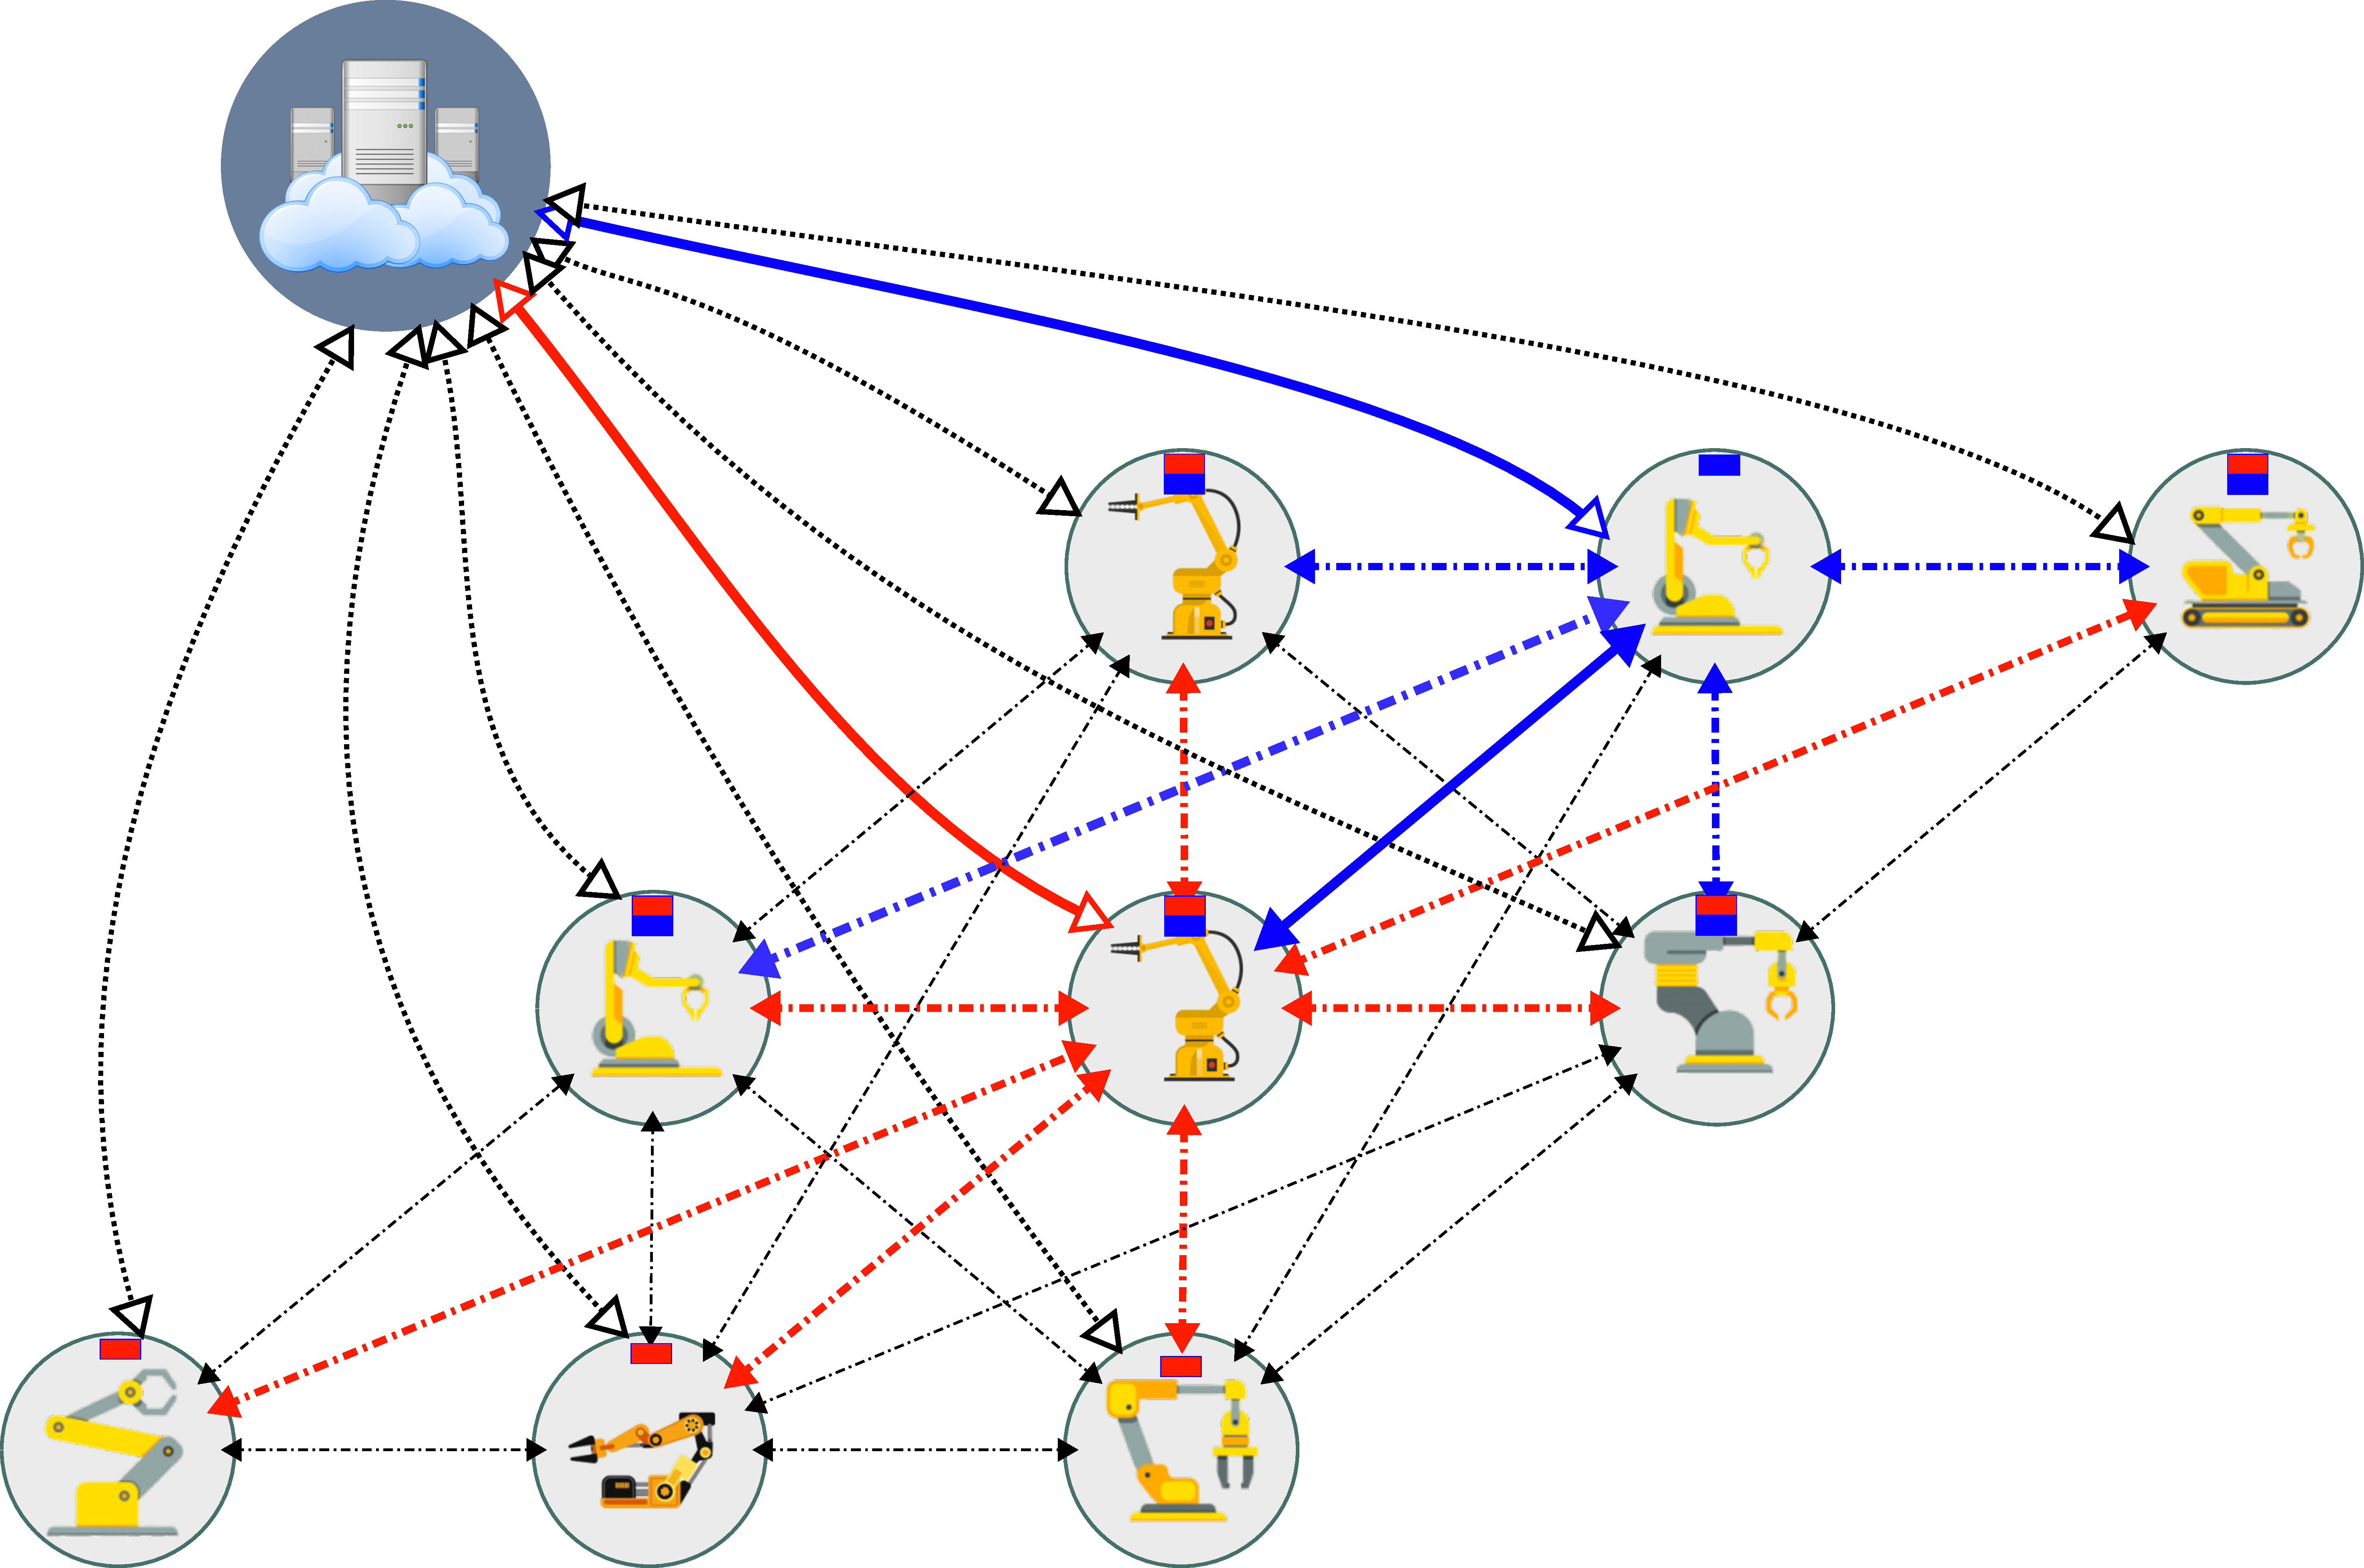
\includegraphics[width=1\columnwidth]{fig/collective_learning_v3.pdf}
%	\caption{How knowledged is transferred, shared, and developed in a collective}
%	\label{fig:collective_learning_v3}
%\end{figure}




%---
%\begin{figure*}[ht!]
%	\centering
%	\hspace*{\fill}
%	\subfloat[]{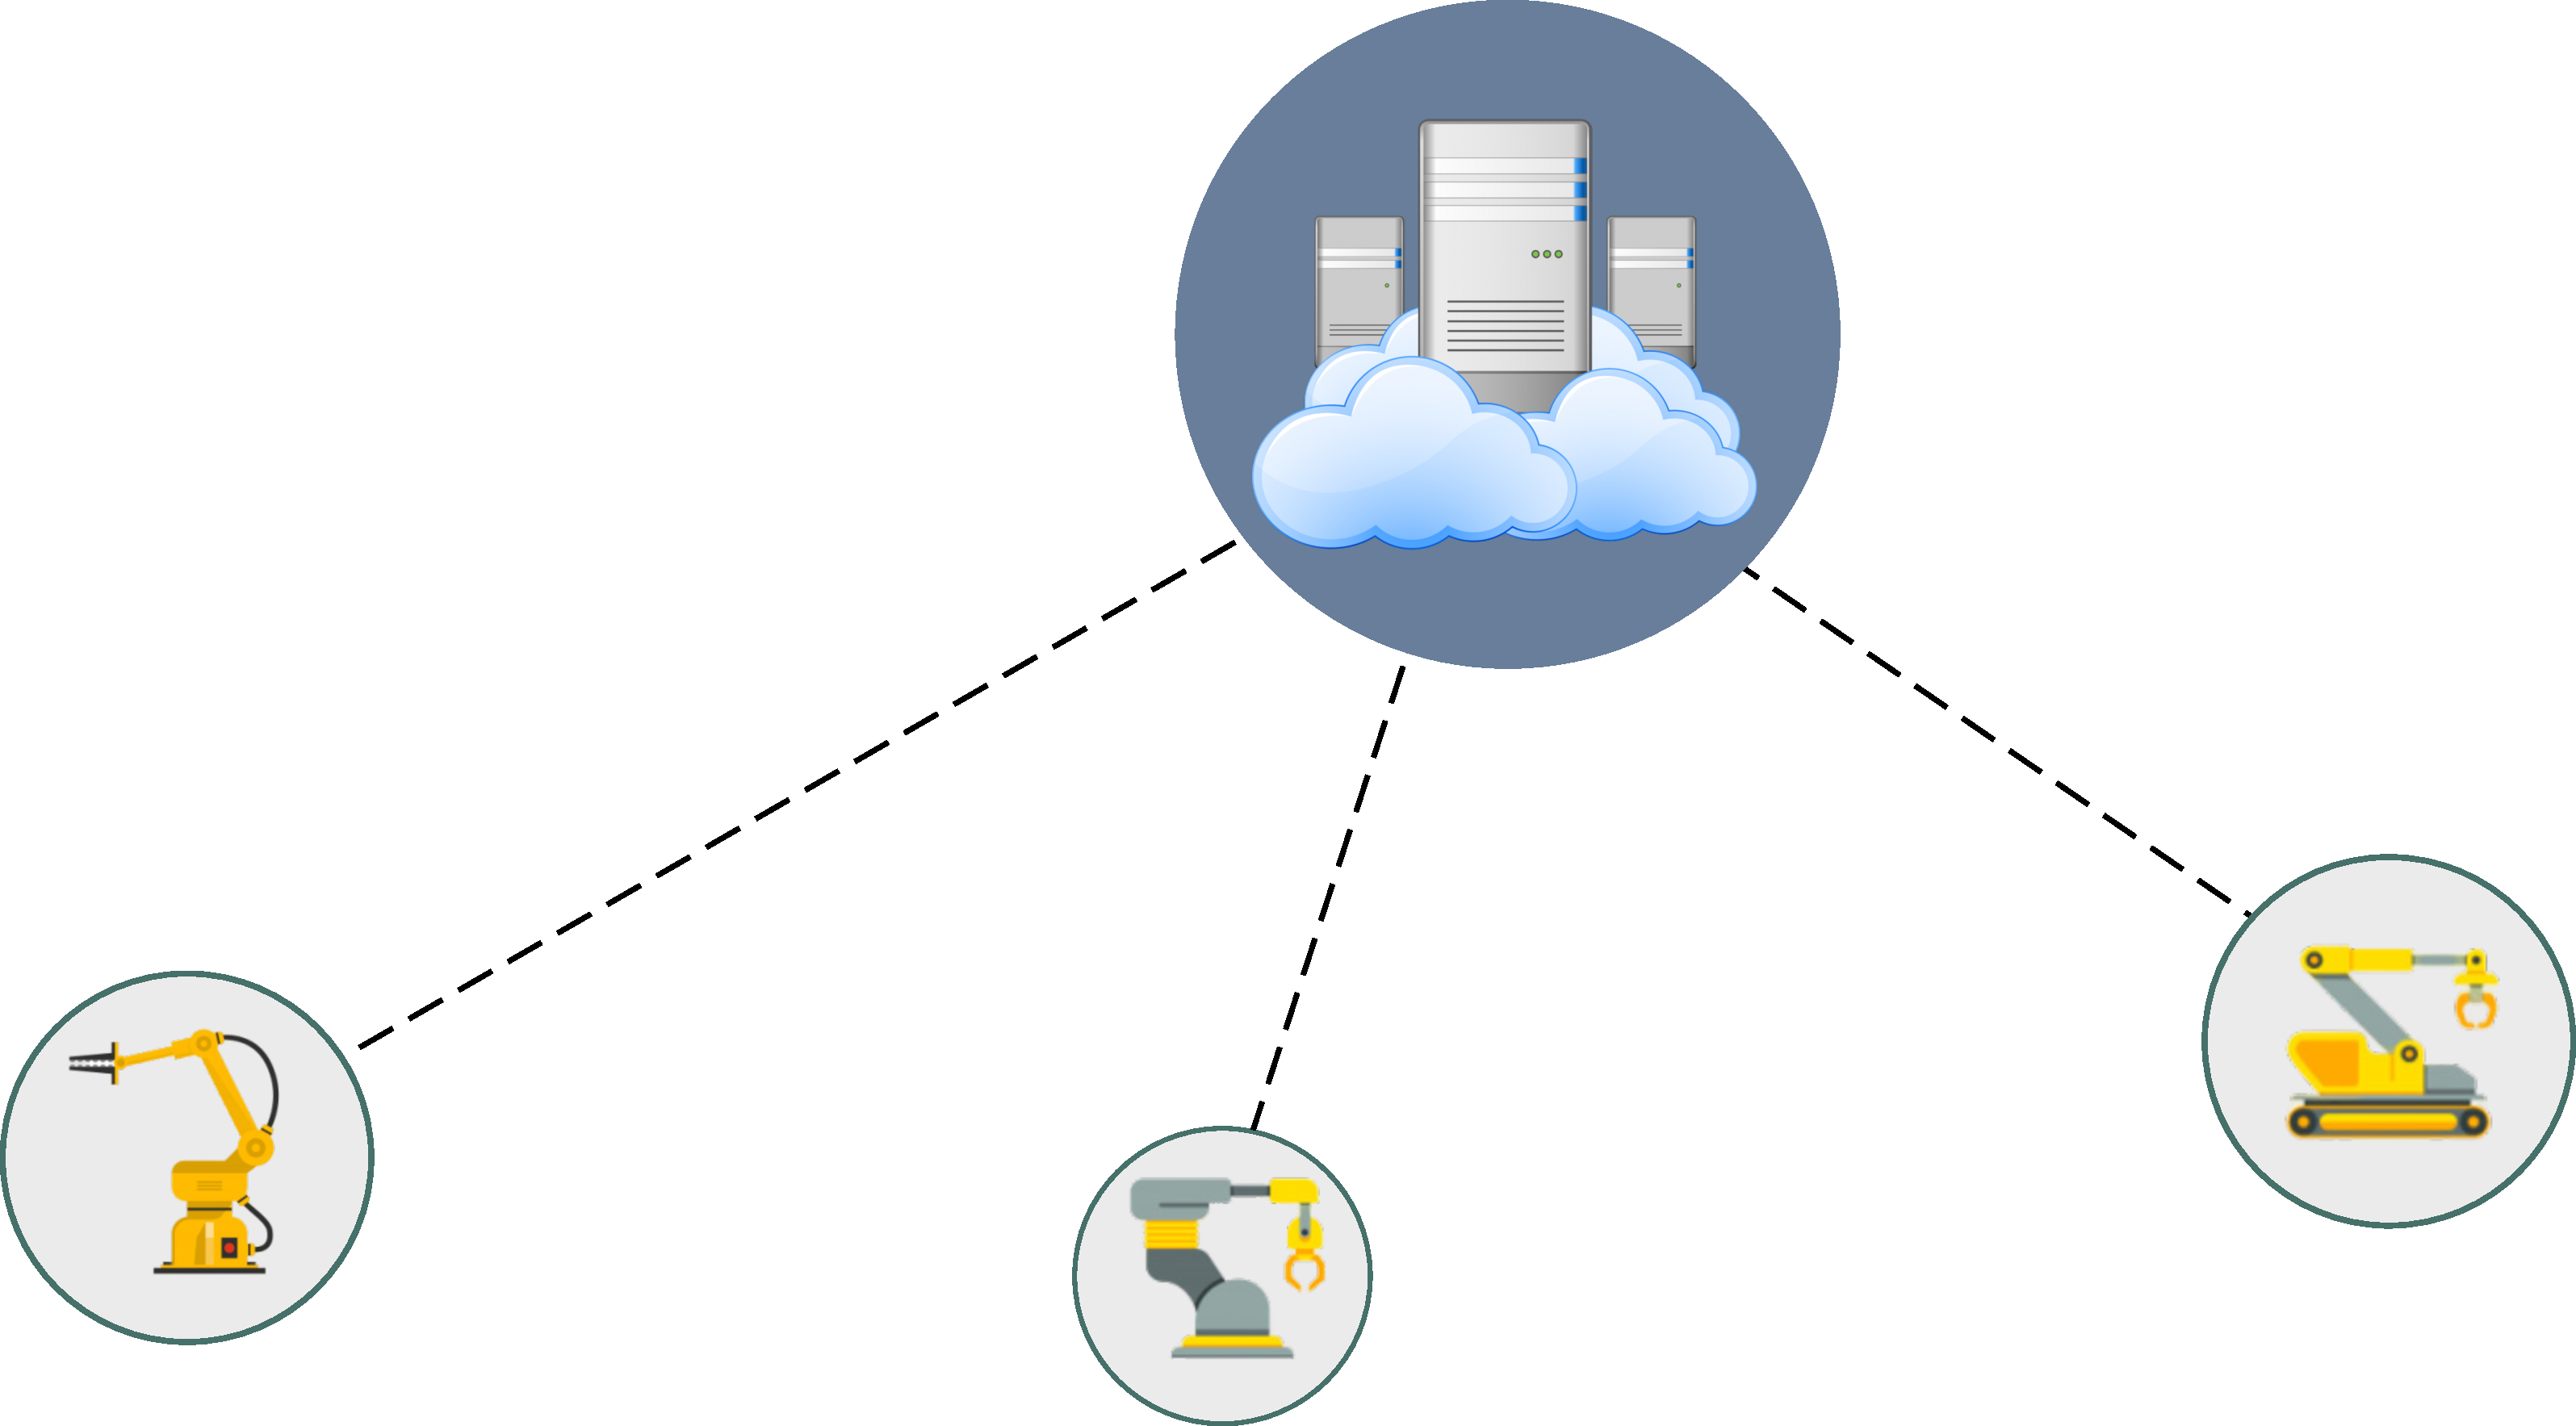
\includegraphics[width= 0.90\columnwidth]{fig/isolated_learning.pdf} \label{fig:isolated_learning}}
%	%\hspace*{\fill}
%	\hfill
%	\subfloat[]{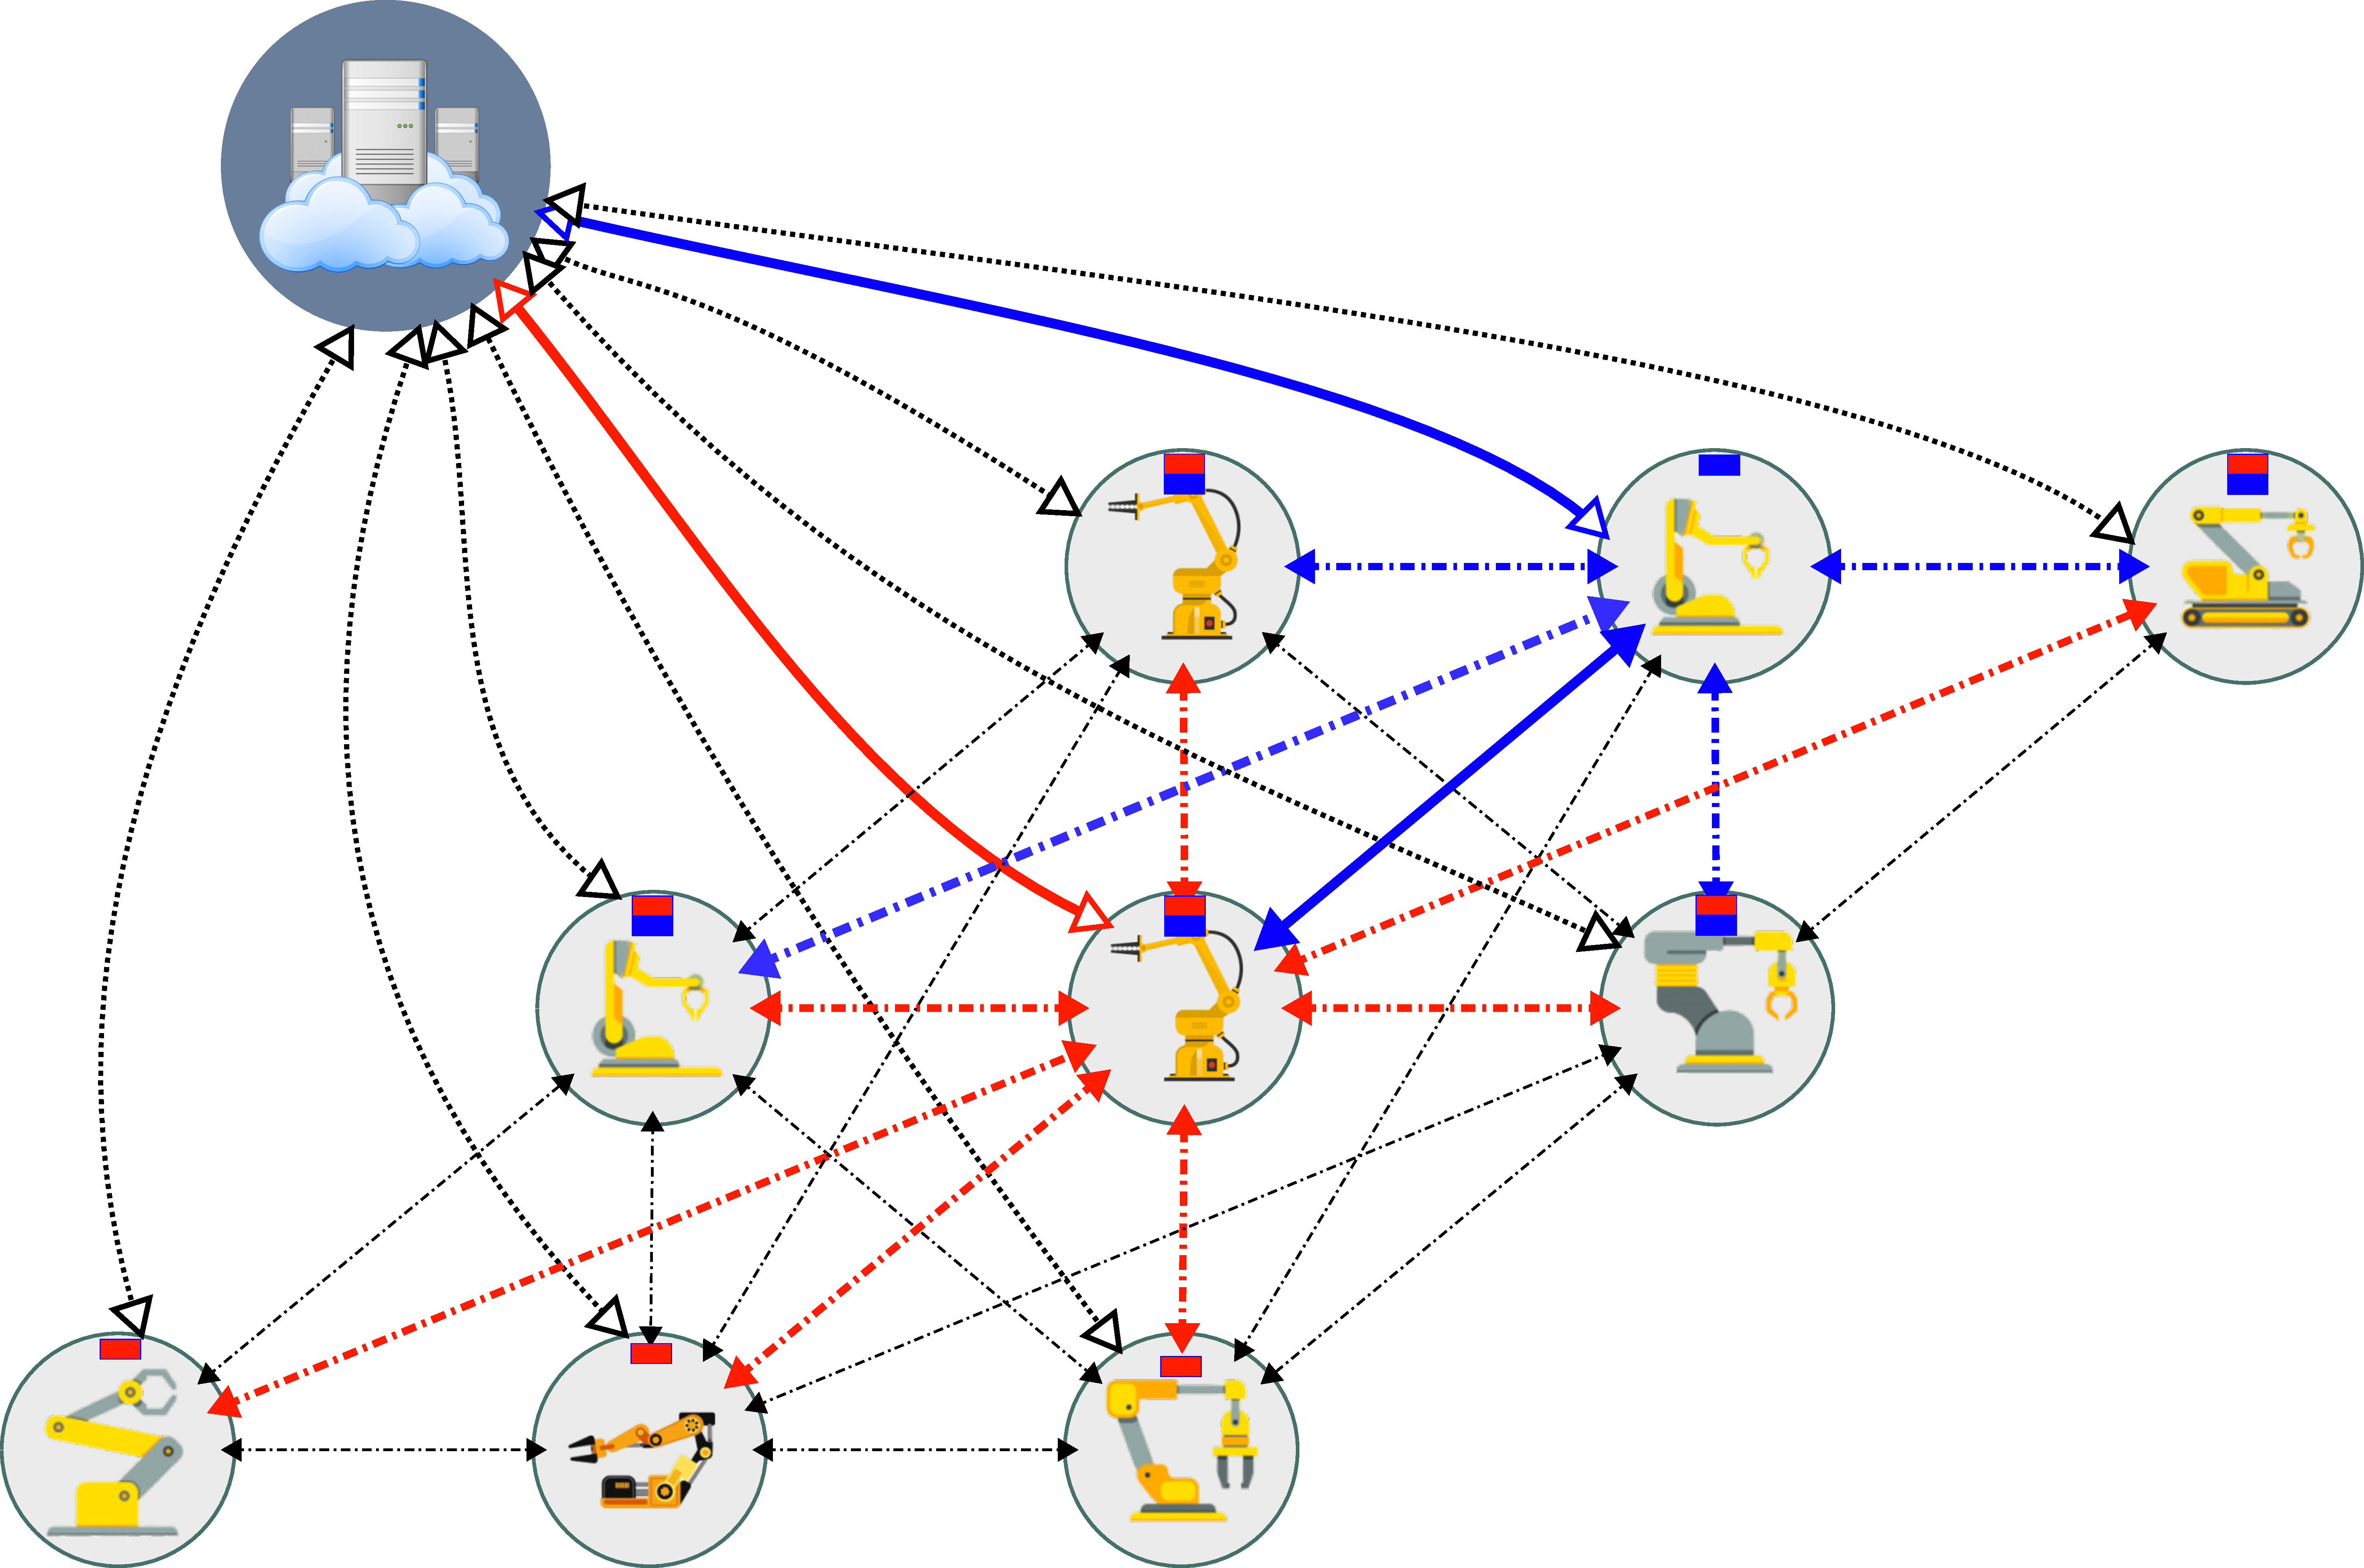
\includegraphics[width= 0.80\columnwidth]{fig/collective_learning_v3.pdf} \label{fig:collective_learning}}
%	\hspace*{\fill}
%	\caption[] {\label{fig:learning_paradigms} Learning paradignms: \subref{fig:isolated_learning} isolated learning and \subref{fig:collective_learning} collective learning. }
%\end{figure*}
%%---

%%---
%\begin{figure*}[ht!]
%	\centering
%	\hspace*{\fill}
%	\subfloat[]{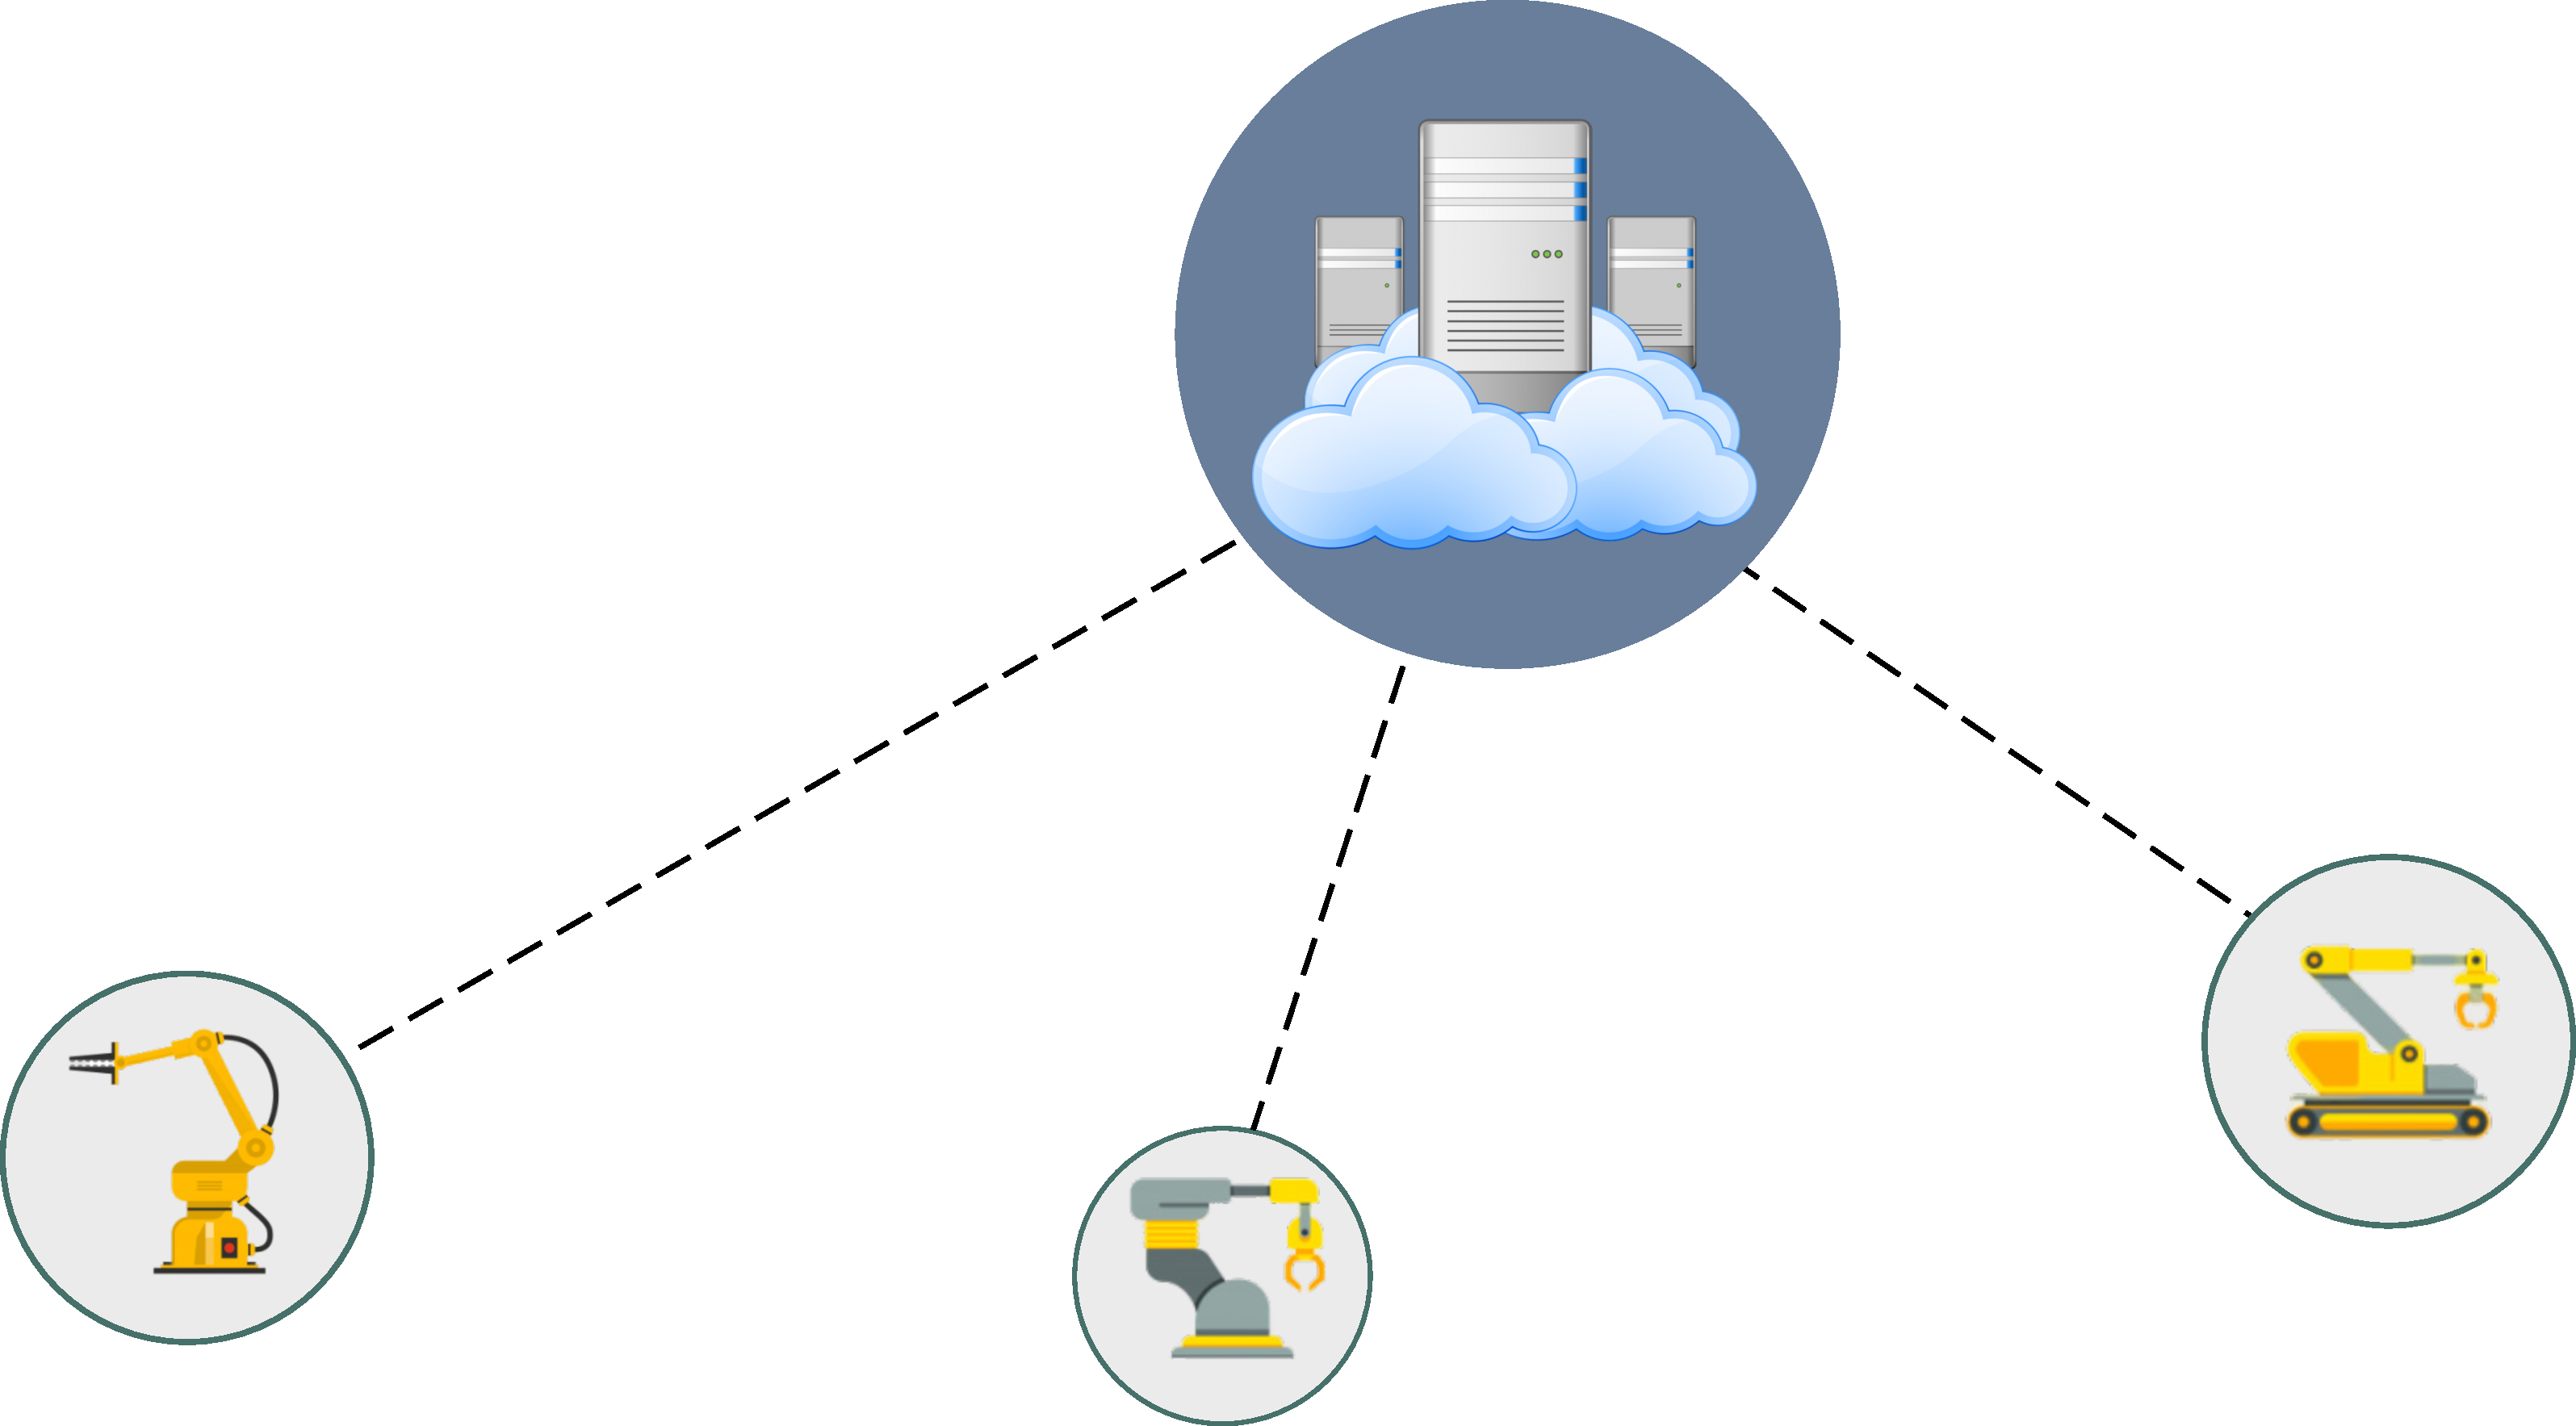
\includegraphics[width= 0.90\columnwidth]{fig/isolated_learning.pdf} \label{fig:isolated_learning}}
%	%\hspace*{\fill}
%	\hfill
%	\subfloat[]{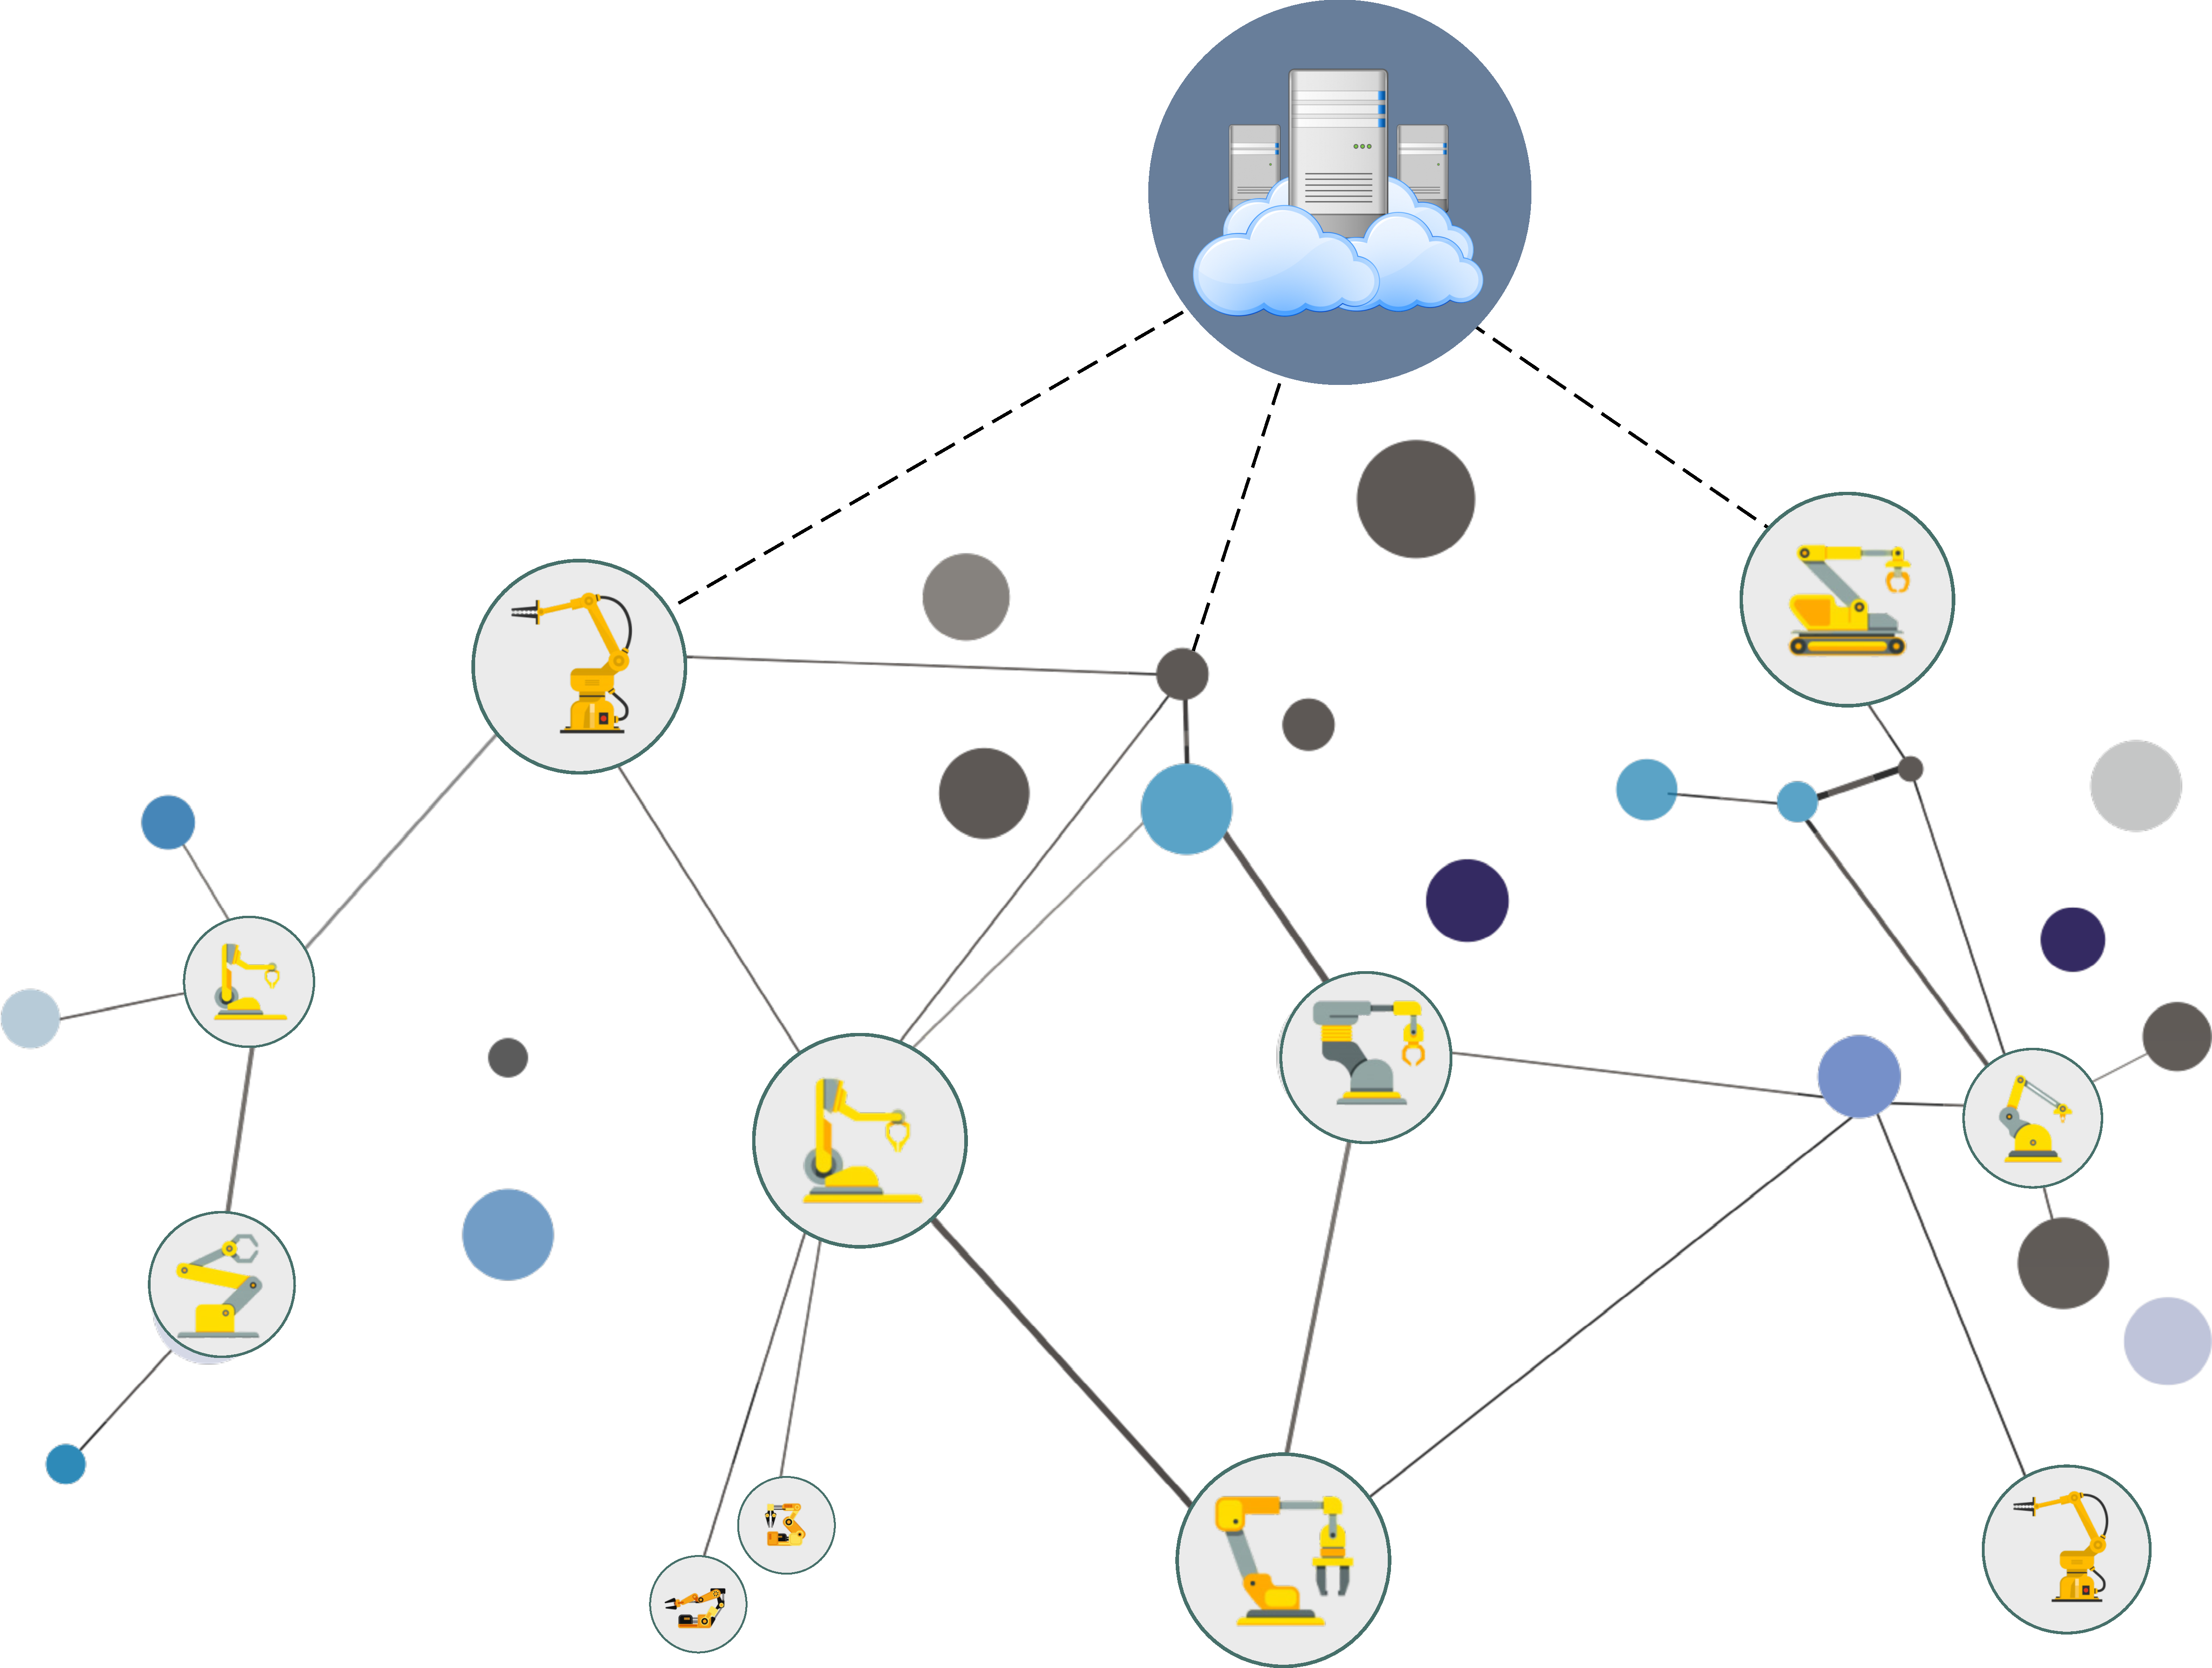
\includegraphics[width= 0.80\columnwidth]{fig/collective_learning.pdf} \label{fig:collective_learning}}
%	\hspace*{\fill}
%	\caption[] {\label{fig:learning_paradigms} Learning paradignms: \subref{fig:isolated_learning} isolated learning and \subref{fig:collective_learning} collective learning. }
%\end{figure*}
%%---


%The ability to share information so efficiently that the ideas of individuals can be stored within the collective memory of communities and can accumulate through generations. 
%
%The process through which different actors develop a collective mind which concerns how they use their own network and interactions as culture-based contextual conditions for everyday learning processes including opportunities to use their concrete experiences, knowledge, and skills. It involves horizontally based cooperation between different actors in a local or organizational setting or the mobilization of resources in a broader context as such to initiate a learning-based process of innovation and change
%
%Collective learning is a complex concept that is variously defined. It is generally conceptualized as a dynamic and cumulative process that results in the production of knowledge. Such knowledge is institutionalized in the form of structures, rules, routines,norms, discourse, and strategies that guide future action. Learning emerges because of interactive mechanisms where individual knowledge is shared, disseminated,  diffused,  and  further  developed  through relational and belonging synergies. 
%
%Collective learning, therefore, represents a macro concept that addresses learning at the levels of the team,the organization, and society. 
%
%An important distinction is made between individual learning and collective learning. Individual learning tends to be conceptualized as an information system where learning is interpreted, retained, and retrieved by individuals. Collective learning is viewed as a more macro-level concept that emphasizes the synergy and advantages of the collective element
%
%Central to collective learning is the notion that the collective is enhanced in three ways: (a) it achieves the capacity to restructure and to meet changing conditions; (b) it can add and use skills, knowledge, and behaviors; and (c) it becomes highly sophisticated in its capability to deal with feedback and reflect on its actions.
%
%Different types of collective learning are highlighted in the literature:
%\begin{itemize}
%	\item Aggregate learning is conceptualized as the aggregation of learning gained though trial and error at the individual level. The emphasis is on individual learning processes rather than any collective perspective. Aggregate learning may give rise to fragmentation and individualization rather than inclusion and collectivity
%	\item Group learning focuses on the processes that a group uses to acquire new skills, knowledge, ways of interacting, change patterns between group members, standard operating procedures, and behavioral routines
%\end{itemize}
%
%Camagni (1991) suggests that collective learning is not simply the acquisition of information, and that the availability of information is not a central issue.Instead, it is the process by which available information becomes usable knowledge that is the main focus.